\documentclass[10pt, conference]{IEEEtran}

\makeatletter
\pdfminorversion=4
\usepackage[margin=0.75in]{geometry}
\usepackage{ifpdf}
\usepackage{cite}
\bibliographystyle{unsrt}
\usepackage{amsmath}
\usepackage{amssymb}
\usepackage{algorithm}
\usepackage[noend]{algpseudocode}
\usepackage{multirow}
\ifCLASSINFOpdf
   \usepackage[pdftex]{graphicx}
\else
\fi
\usepackage{upgreek}
\usepackage{dblfloatfix}
\usepackage{xcolor}
\usepackage{hyperref}
\usepackage{soul}
\usepackage{hhline}
\usepackage{booktabs}
\usepackage{float}
\hypersetup{
    colorlinks=true,
    linkcolor=blue,
    filecolor=magenta,
    urlcolor=cyan,
    citecolor=cyan,
}
\IEEEoverridecommandlockouts

\setlength{\textfloatsep}{1\baselineskip plus 0.2\baselineskip minus 0.5\baselineskip}

\newcommand{\cdo}[1]{\textcolor{red}{CDO: #1}}
\newcommand{\jx}[1]{\textcolor{blue}{JX: #1}}
\newcommand{\sh}[1]{\textcolor{orange}{SH: #1}}

% --- review markup: proposed cuts -----------------------------------------
% \cut{...}     strikes prose;  \cutmath{...} strikes a display equation
% \cutwhy{...}  the reason, in gray, beside the struck text
% Delete these three macros and the struck text once the cuts are accepted.
\usepackage[normalem]{ulem}
\newcommand{\cut}[1]{\textcolor{gray}{\sout{#1}}}
\newsavebox{\cutbox}
\newcommand{\cutmath}[1]{\textcolor{gray}{%
  \sbox{\cutbox}{$\displaystyle #1$}%
  \rlap{\usebox{\cutbox}}\rule[0.45ex]{\wd\cutbox}{0.5pt}}}
\newcommand{\cutwhy}[1]{{\color{gray}\footnotesize\itshape [#1]}}

% Citation placeholders for papers not yet in references.bib.
\newcommand{\isrr}{\sh{[cite ISRR 2026]}}
\newcommand{\iros}{\cite{hyland_before_2026}}

\renewcommand\IEEEkeywordsname{Keywords}

% TITLE OPTIONS (pick one, keep "Probing for Properties"):
%   - (previous main.tex title) Probing for Properties
%   - Probing for Properties: Touch Once, Then Shove
%   - Probing for Properties: Non-Prehensile Estimation that Predicts Its Own Failures
%   - Feel Before You Shove: Choosing, Executing, and Trusting Non-Prehensile Probes of Mass, CoM, and Friction
%   - (outline) Probing for Properties: Certified Non-Prehensile Estimation of Mass, Center of Mass, and Friction, and Their Use in Manipulation
\title{\LARGE \bf Probing for Properties: Choosing, Executing, and Trusting Non-Prehensile Probes of Mass, Center of Mass, and Friction}

\begin{document}

\author{Steven M. Hyland, Jing Xiao, and Cagdas D. Onal \\ \thanks{The authors are affiliated with the Robotics Engineering Department, Worcester Polytechnic Institute, MA 01609, USA. Correspondence: \texttt{smhyland@wpi.edu}.}}

\maketitle
\pagestyle{plain}
\thispagestyle{plain}

\begin{abstract}
% NOTE: results-agnostic. Fill the orange placeholders from the journal experiments.
Safe manipulation depends on a small set of physical parameters, mass, center of mass (CoM), and the object--surface friction coefficient, that together decide whether an applied force slides an object, tips it, or knocks it over, and that cannot be read reliably from vision alone. We show that a robot can decide where to touch an object it has never seen, which non-prehensile primitive will actually work on it, and how far it can safely drive that primitive, using only a partial point cloud and a wrench signal, with no shape model and nothing learned. Contact points for both forward tipping and press-and-pull tipping are chosen by a single torque objective over the point cloud, and the tipping mode is chosen by a three-step heuristic that predicts base instability, sliding, and press-point usability before contact and verifies them during contact. Both modes share one estimator, which recovers the mass-weighted first moments of the CoM about the pivot from a single tip, and mass and CoM height given the planar CoM; a side camera labels what the object did while proprioception measures how far it tilted. Press-induced table slip is treated as the single governing hazard of press-and-pull, so the arc can be driven past the balance point when the object allows it. We characterize where the method stops working with controlled sweeps over CoM offset, base rounding, and base friction on \sh{N} objects and configurations, and propagate measurement uncertainty from the wrench and point cloud into the estimates. Finally, we show the numbers are worth having: the estimates plan a dynamic shove-to-region task in closed form, predicting before any motion which shoves will land the object in the goal and which will tip it, including on objects whose exteriors are identical. \sh{Headline numbers: mass error X\%, CoM height error Y\%, shove success Z/N vs. uninformed policies.}
\end{abstract}

\begin{IEEEkeywords}
Force and Tactile Sensing, Contact Modeling, Perception for Grasping and Manipulation, Non-Prehensile Manipulation
\end{IEEEkeywords}

\IEEEpeerreviewmaketitle

%% ==============================================
\section{Introduction} \label{sec:intro}
%% ==============================================

Robots increasingly handle objects without grasping: a toolbox nudged into place, a monitor too large to pick up, a package rebalanced on a shelf. Whether such manipulation succeeds safely is governed by a compact set of physical parameters: the object's mass $m$, its center of mass (CoM), and the friction coefficient $\mu_t$ at the object--table contact. Together, these decide whether an applied wrench tips an object, slides it, or leaves it stationary. None of them is reliably observable from vision: a textureless casing, a hollow shell, and a box of identical appearance with its weight up front can carry entirely different mass distributions.

While the parameters cannot be seen, they can be probed. Non-prehensile primitives such as pushing and tipping need no grasp planning, no fixturing, and no prior geometric model, and they apply precisely to the objects that grasping cannot reach. Planar pushing recovers only the planar CoM $(x_c, y_c)$ and cannot separate mass from friction \cite{mason_mechanics_1986, bauza_probabilistic_2017, hyland_predicting_2023}. Tipping recovers the third CoM coordinate and the mass, but operates near an inherently unstable boundary. Our prior work developed forward tipping \iros{}, a force-guided single-push tip that recovers $z_c$ and $m$ but fails on low-friction and curved bases, and press-and-pull tipping \isrr{}, which presses down while pulling to keep such objects from sliding and to pin the pivot, and which recovers friction when sequenced with a planar slide.

Those papers left the questions that decide whether non-prehensile estimation is usable on an object nobody has characterized: where to place the contact, which tipping mode will actually work, how hard to press and how far to tip without losing control of the object, where the method stops working, and whether the recovered numbers are good enough to act on. The ISRR paper gives rules for the press point without reasoning or validation, and lists a feasible object set without quantitatively characterizing its boundaries. \sh{ISRR named three extensions and left two questions open; this paper delivers four of those five, leaving only object compliance (liquid estimation) for future work. List them explicitly here.}


% THIS FIGURE IS NO LONGER REALLY APPLICABLE. WE ARE NOT PURELY ANALYZING PRESS-PULL TIPPING...
% \begin{figure}[t]
%   \centering
%   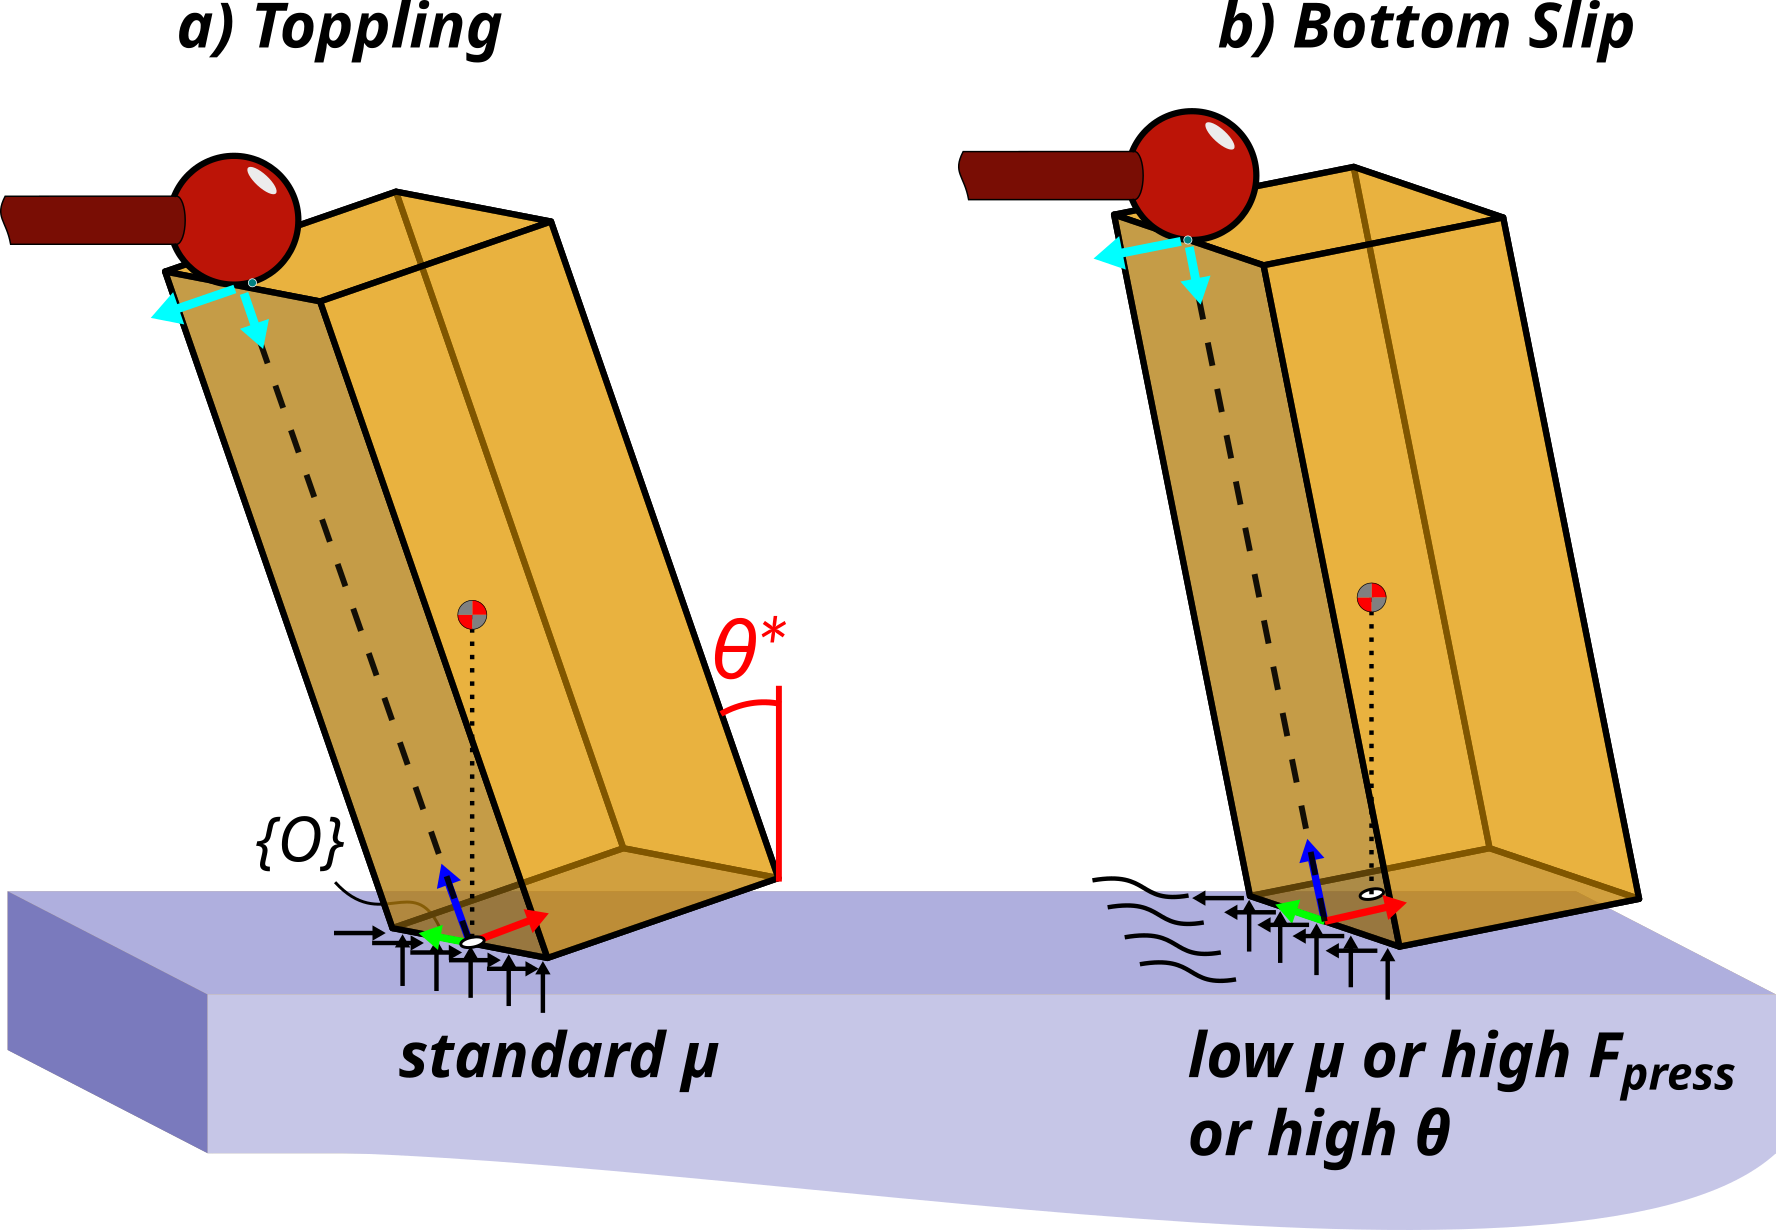
\includegraphics[width=0.95\linewidth]{figures/safety_cases.png}
%   \caption{The two hazards of press-and-pull tipping. (a) Toppling: past the toppling angle $\theta^{*}$ the CoM crosses the pivot and gravity continues the rotation. (b) Bottom slip: a low $\mu_t$, a large press $F_{\mathrm{press}}$, or a large tip angle $\theta$ drives the base to slide. We show in Section~\ref{sec:method} that (a) is a consequence of (b), so only slip needs to be certified. \sh{Figure is from the old draft; keep, but check notation matches $\eta_{\mathrm{slip}}$.}}
%   \label{fig:hazards}
% \end{figure}

\noindent\textbf{The claim, in one sentence.} A robot can decide where to touch an unknown object, which non-prehensile primitive will work on it, and how far it can safely drive that primitive, using only a point cloud and a wrench signal, with no shape model and nothing learned, and the parameters it recovers this way are accurate enough to plan a dynamic task whose failure modes are predicted in advance.

The paper is organized around four pieces (Table~\ref{tab:contributions}):

\begin{itemize}
  \item \textbf{C1, choosing the contact and the tipping mode.} Press and push points become a stated optimization over the point cloud rather than a rule of thumb, with the trade between contact height and distance to the pivot set by fingertip friction rather than by hand. A three-step heuristic chooses forward tipping or press-and-pull from predicted base instability, predicted and observed sliding, and press-point usability.
  \item \textbf{C2, keeping the interaction safe.} One governing hazard (table slip), a bounded band of safe press forces, and a margin $\eta_{\mathrm{slip}}$ that permits deliberately tipping past the balance point when the object allows it. Forward tipping is guarded by a stopping rule, a slide probe, and an observability gate that needs no prior.
  \item \textbf{C3, saying where the method stops working.} Controlled sweeps over CoM offset, base rounding, and base friction (bottom material), each with a degradation curve and a stated breakdown point, together with uncertainty propagated from the wrench and point cloud through the estimator.
  \item \textbf{V, showing the numbers are worth having.} A dynamic shove into a target region, planned in closed form from the estimates, with a no-tip push-height window, a coast-phase gate, and a release condition, compared against uninformed push policies.
\end{itemize}

\begin{table}[t]
  \centering
  \caption{The four pieces of the paper and what backs each one.}
  \label{tab:contributions}
  \small
  \begin{tabular}{p{0.06\linewidth} p{0.40\linewidth} p{0.40\linewidth}}
    \toprule
    & \textbf{Contribution} & \textbf{Evidence} \\
    \midrule
    C1 & Contact and tipping-mode choice & Contact-placement ablation; mode choice against outcome for every object \\
    C2 & Keeping the interaction safe & Per-tip margin traces; retry and failure rates; safety--accuracy curve \\
    C3 & Where the method stops working & Degradation curves and breakdown points per swept axis; uncertainty budget and coverage \\
    V & The numbers are worth having & Predicted vs.\ observed shove outcomes for four push policies \\
    \bottomrule
  \end{tabular}
\end{table}

A single principle runs through all four: \emph{more affordance from less information}. A robot can recover, and then act on, an unknown object's mass, CoM, and friction using only non-prehensile contact, proprioception, and a partial view, with closed-form reasoning at every step. \sh{Candidate thesis statement; restate in the conclusion. Also decide whether the dissertation mapping (planar pushing $\rightarrow$ forward tipping $\rightarrow$ press-and-pull $\rightarrow$ this paper) belongs in the intro or only in the dissertation.}

The press-and-pull primitive, forward tipping, and the multi-modal $(m, z_c, \mu_t)$ decomposition are carried from our prior work \iros{}, \isrr{} and recapped in Section~\ref{sec:background}; they are not claimed as new here. The planar CoM comes from our earlier pushing work \cite{hyland_predicting_2023, hyland_onboard_2025} and is cited, not re-derived.

%% ==============================================
\section{Prior Work} \label{sec:prior}
%% ==============================================

\noindent \textbf{Inertial parameter estimation through interaction.} Identifying inertial parameters by exciting an object and observing the resulting wrench has a long history, from rigid-body identification of manipulator payloads \cite{atkeson_rigid_1985, khosla_parameter_1985} to in-hand estimation of grasped objects \cite{kubus_-line_2007, sundaralingam_-hand_2021}. Mavrakis and Stolkin \cite{mavrakis_estimation_2020} survey the space along contact model, sensing modality, and active-versus-passive estimation. Most of this work assumes a secure grasp, which excludes precisely the objects that motivate non-prehensile manipulation. We treat the object--table contact not as something to be eliminated by grasping but as a \emph{passive grasp} in the wrench balance. The payload literature also gives us the right language for what a single tip can and cannot identify: as in base-parameter identification, mass and first moments are identifiable where the CoM alone is not (Section~\ref{sec:identifiability}).

\noindent \textbf{Pushing-based estimation.} Quasistatic planar pushing is a well-studied primitive \cite{mason_mechanics_1986, lynch_estimating_1993, bauza_probabilistic_2017}. A recurring finding is that planar interaction alone cannot disentangle mass from friction: a small number of pushes fixes only their product, leaving a distribution over both \cite{bauza_probabilistic_2017}. Some methods sidestep identification by closing the loop on force feedback \cite{heins_force_2024}; others recover full parameter sets but require learned interaction models \cite{dutta_push_2023}. We activate modes sequentially so that each reveals the parameters it is suited for.

\noindent \textbf{Friction estimation and slip onset.} Friction has classically been estimated through sliding, lateral pressing with tactile sensing, or slip-detection control on grasped objects \cite{sundaralingam_-hand_2021}, with proprioceptive ground-reaction methods used for terrain friction in legged systems \cite{kim_online_2025}, and by observing the resultant motion of pushed objects \cite{lynch_estimating_1993}. We adopt the slip-onset principle but transpose it to a non-prehensile setting, reading friction from the table reaction at incipient slide, including from forward tips that slide rather than tip.

\noindent \textbf{Tipping and toppling.} Tipping has been studied both as a manipulation goal and as an estimation tool. Equi-effect methods recover the CoM by tipping an object about several support lines and intersecting the resulting planes \cite{yong_yu_estimation_1999, yong_yu_estimation_2001, yong_yu_estimation_2005}; they require at least three tips with independent supports, matched contact points, and polyhedral geometry, and do not recover friction. Force-guided single-interaction tipping removes the geometry requirement and the need for repeated tips \iros{}, but fails on low-friction curved bases which slide or swirl before they tip. Press-and-pull \isrr{} resolves that failure with a stabilizing press. None of these choose between modes, and none state where they stop working.

\noindent \textbf{Safety and uncertainty in non-prehensile manipulation.} A separate line of work addresses safety at \emph{execution} time. Robust non-prehensile transport plans against bounded inertial uncertainty rather than estimating it \cite{heins_robust_2025}; model-predictive contact controllers respect friction-cone and non-sliding limits \cite{selvaggio_non-prehensile_2023, heins_keep_2023}; and belief-space planar pushing propagates configuration uncertainty through quasistatic contact dynamics \cite{jankowski_robust_2025}. Classical tip-over stability margins serve the same purpose, from the zero-moment point and the force--angle measure \sh{[cite Papadopoulos and Rey 1996]} to mobile-manipulator descendants such as the moment-height measure \sh{[cite Moosavian and Alipour 2006]}, as does more recent topple-avoiding pushing, whether learned via constrained reinforcement learning \sh{[cite constrained-RL topple-avoiding pushing]} or tuned via Bayesian optimization \sh{[cite BO stable pushing]}. All of the above certify \emph{execution} of a known plan on a (partially) known object. Our concern is instead safety at \emph{estimation} time: keeping the probing interaction that produces the knowledge in the first place safe, with the margin computed from the very quantities being estimated.

\noindent \textbf{Vision, learning, and VLM priors.} Learned and vision-based methods predict physical properties from appearance \cite{xu_densephysnet_2019} or refine VLM-inferred priors with interaction \cite{wang_phys2real_2026}. Our method is closed-form throughout, which is a deliberate position: every decision the robot makes can be traced to a stated inequality, and every failure to a violated assumption. \sh{Keep the qualitative capability table from OLDmain (Table method\_comparison); re-verify the Phys2Real marks.}

\noindent \textbf{Positioning.} Our work is most closely related to forward tipping \iros{}, press-and-pull \isrr{}, and multi-tip equi-effect estimation \cite{yong_yu_estimation_1999}. Relative to these, we (i) choose the contact and the mode from the point cloud with stated objectives, (ii) treat press-induced slip as the single governing hazard and allow crossing the toppling angle, (iii) characterize the operating envelope numerically, and (iv) close the loop on a dynamic shove. The downstream shove is adjacent to, but distinct from, the classical pushing literature: quasistatic stable pushing \cite{mason_mechanics_1986, lynch_manipulation_1992} and the pusher--slider line \cite{zhou_pushing_nodate} are planar and controllability-focused rather than tipping-aware, and dynamic pushing \cite{lynch_dynamic_1996} and robust transport \cite{heins_robust_2025} plan around inertial parameters rather than consuming an online estimate. The underlying tipping mechanics are classical; our contribution is assembling them into a parameter-gated feasibility check rather than a new pushing theory.

%% ==============================================
\section{Background} \label{sec:background}
%% ==============================================

This section recaps the forward-tipping and press-and-pull models from \iros{} and \isrr{} to the extent needed for the rest of the paper. We assume throughout a rigid body (or a mildly compliant one, as the monitor in \isrr{}), quasistatic motion during estimation, and a single isotropic Coulomb friction coefficient $\mu_t$ at the object--table contact.

\begin{figure*}[t]
  \centering
  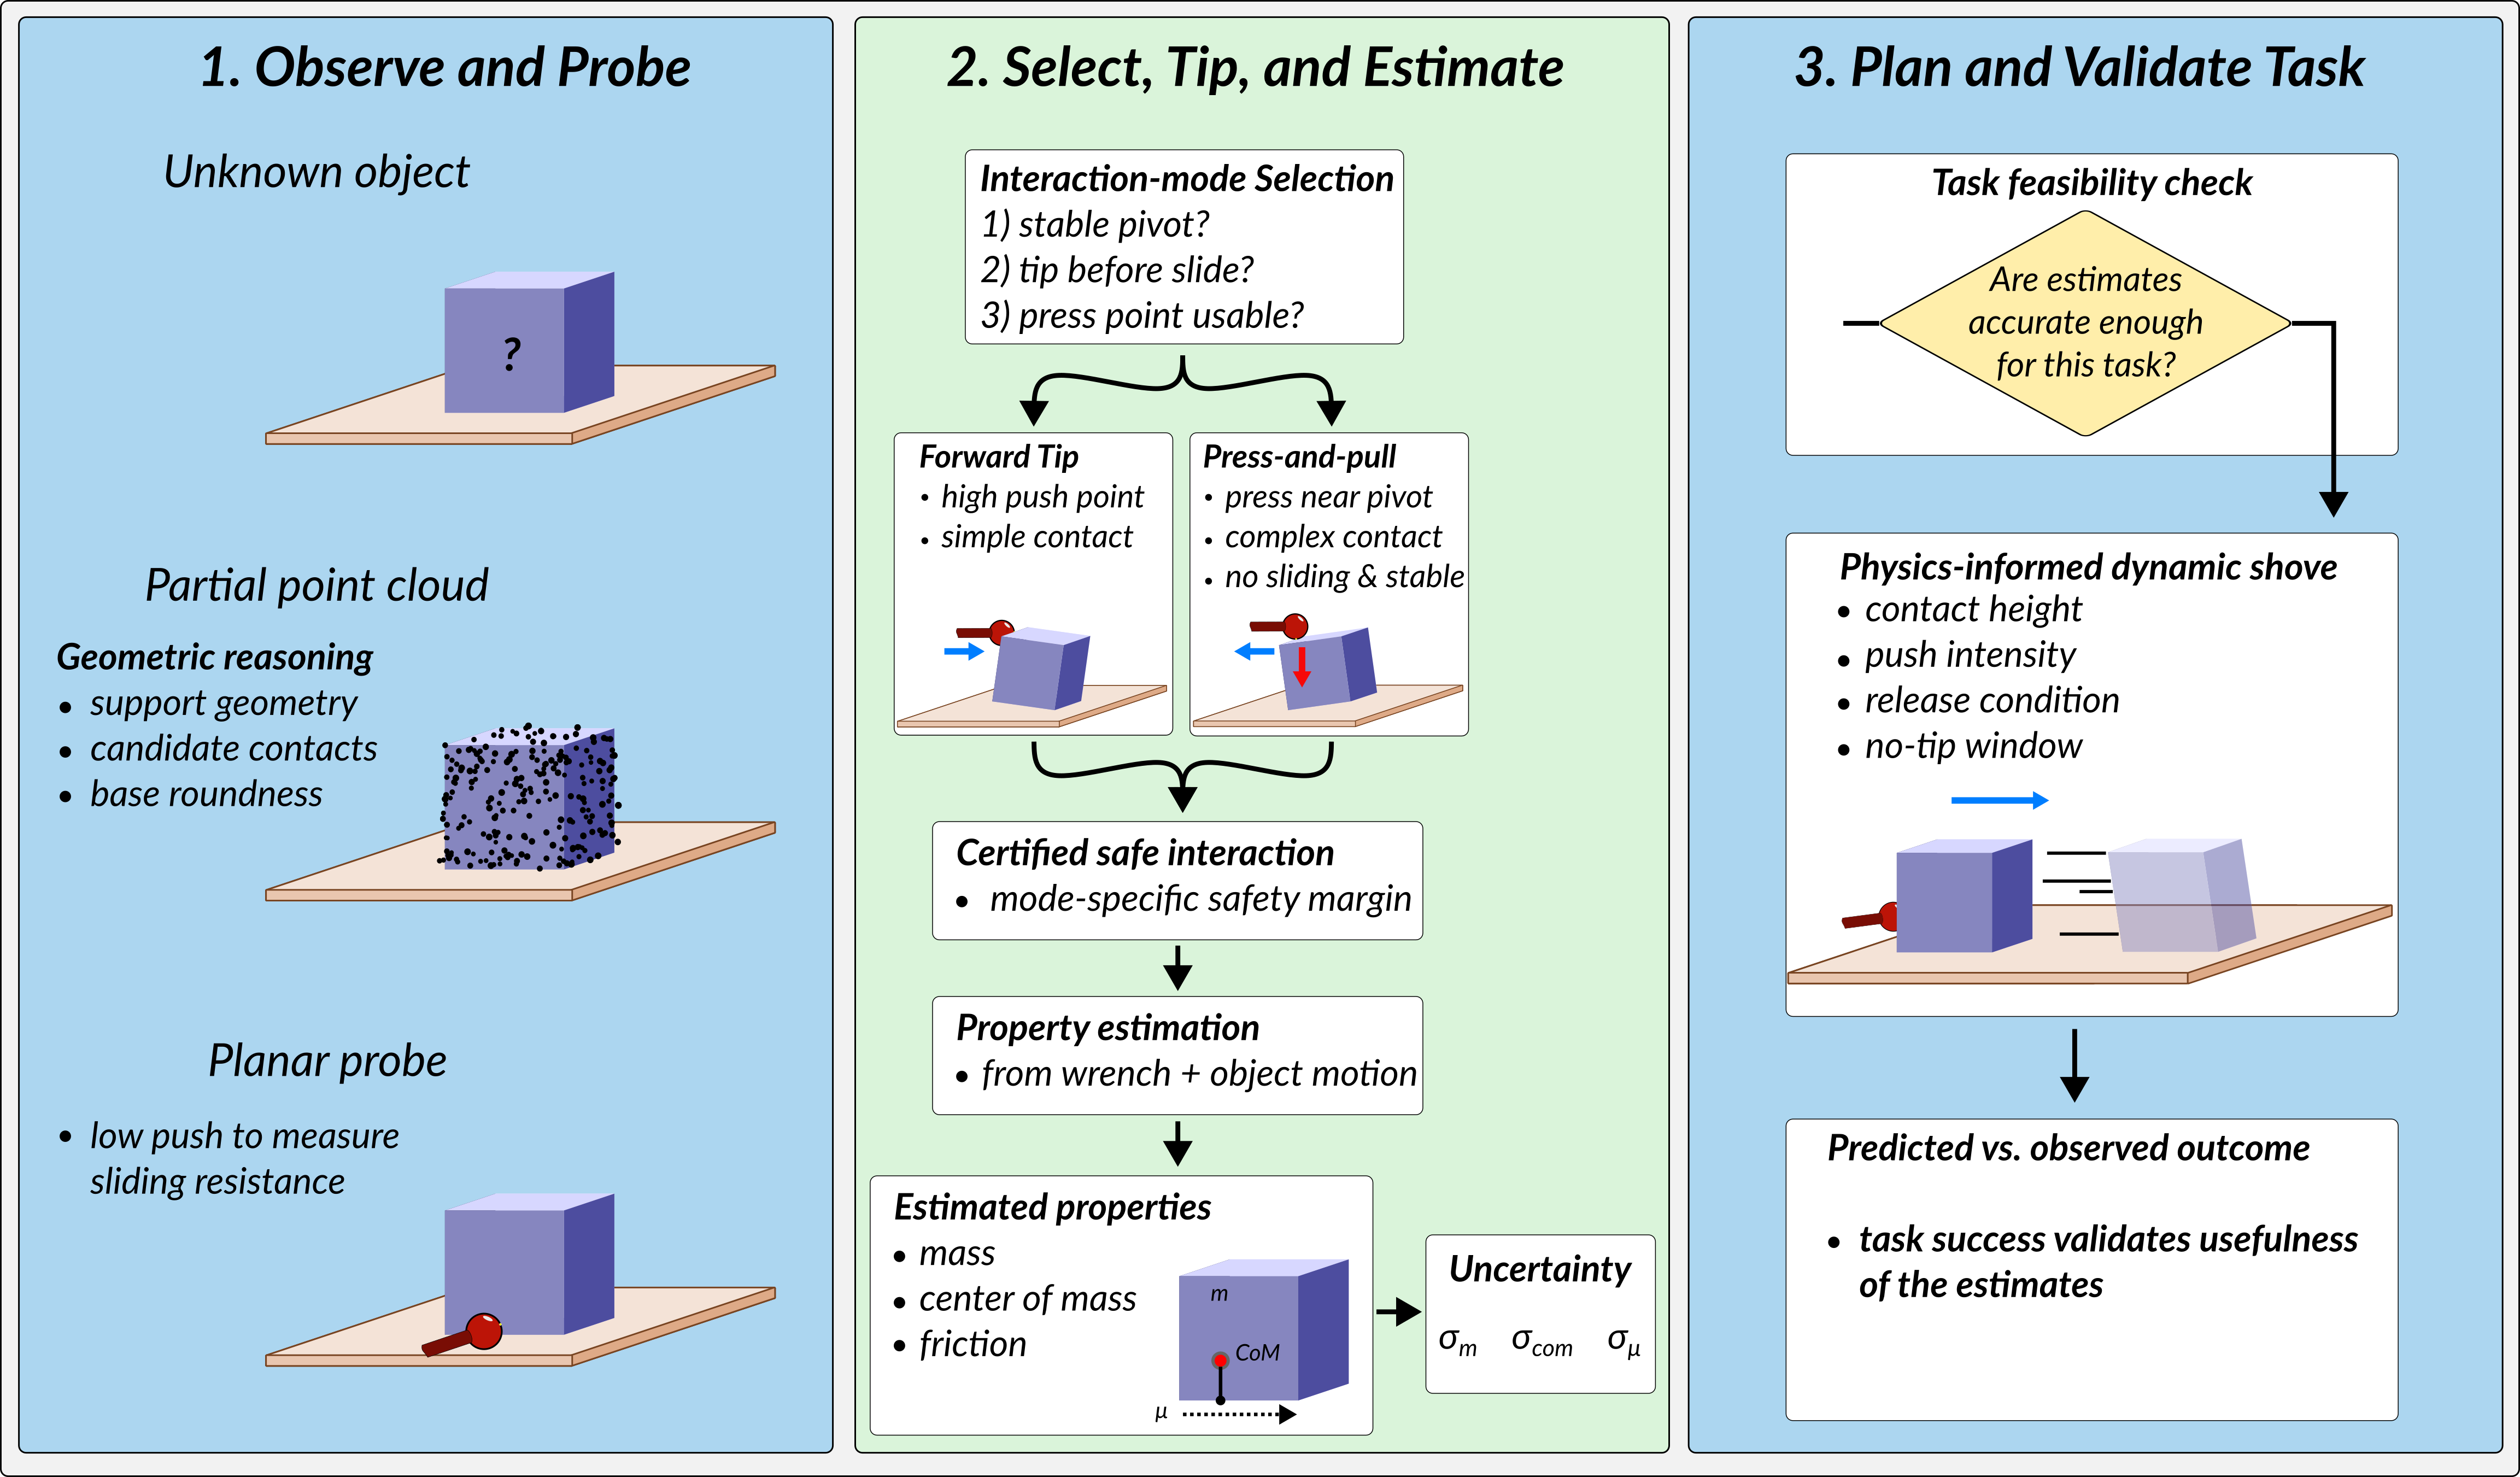
\includegraphics[width=0.95\textwidth]{figures/flowchart_new.png}
  \caption{The full pipeline. (1) Observe and probe: from a partial point cloud the robot reasons about support geometry, candidate contacts, and base roundness, and a low planar push measures sliding resistance. (2) Select, tip, and estimate: the mode heuristic (stable pivot? tip before slide? press point usable?) chooses forward tipping or press-and-pull, the interaction runs inside a mode-specific safety margin, and one shared estimator recovers $m$, the CoM, and $\mu_t$ with uncertainty. (3) Plan and validate a task: a feasibility check asks whether the estimates are accurate enough for the task, a physics-informed shove chooses contact height, intensity, and release, and predicted outcomes are compared against observed ones.}
  \label{fig:flowchart}
\end{figure*}

% DEPRECATED IN FAVOR OF NEW FLOWCHART
% \begin{figure}[t]
%   \centering
%   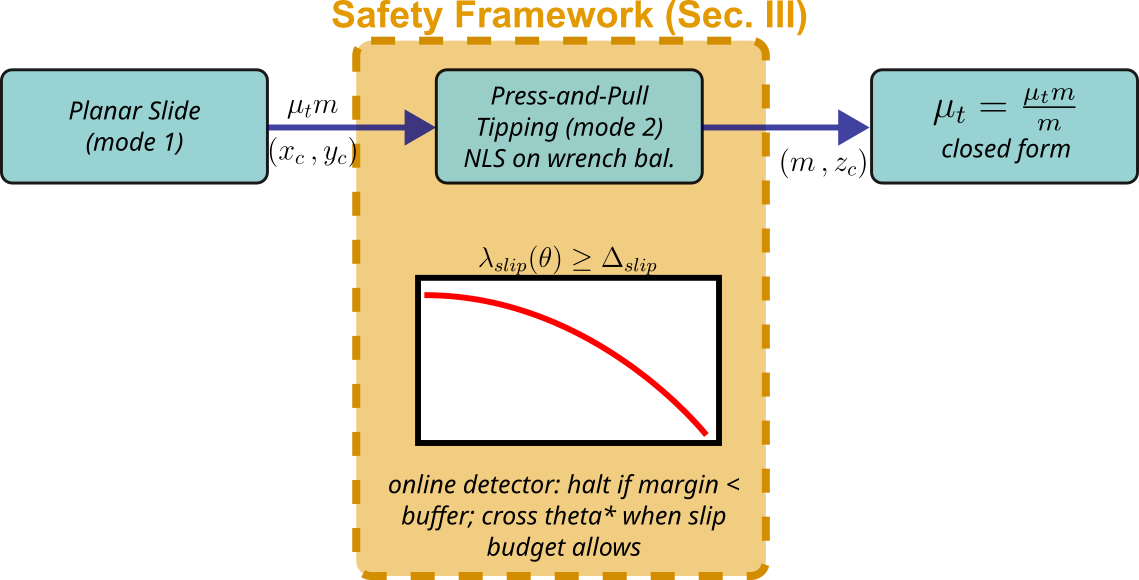
\includegraphics[width=0.95\linewidth]{figures/pipeline.png}
%   \caption{Multi-modal pipeline (old draft). A planar slide caches the product $\mu_t m$ and supplies planar CoM $(x_c, y_c)$; press-and-pull tipping recovers $(m, z_c)$ via nonlinear least squares on the wrench balance; friction is then recovered in closed form. \sh{SUPERSEDED by Fig.~\ref{fig:flowchart}; delete this figure (and figures/fig2\_pipeline.png, its synthetic twin) once the flowchart is accepted.}}
%   \label{fig:pipeline}
% \end{figure}

\noindent \textbf{Forward tipping.} Let $\{O\}$ be the object frame located on the pivot edge and $\varphi$ the object's out-of-plane rotation about that edge. A horizontal push at height $h$ tips the object about the far edge. At a fixed pivot the quasistatic torque balance
\begin{equation}
    {}^{O}\mathbf{p}_{\mathrm{push}}\times{}^{O}\mathbf{F}_{\mathrm{push}}
    + {}^{O}\mathbf{p}_{c}\times{}^{O}\mathbf{F}_{\mathrm{grav}} = \mathbf{0}
    \label{eq:torque_balance}
\end{equation}
recovers the CoM parameters, with $\mu_t$ structurally absent: tipping is friction-agnostic by construction. Whether an object tips at all is decided by the competing onset thresholds
\begin{equation}
  F_{\mathrm{slide}} = \mu_t N, \qquad
    F_{\mathrm{tip}} = \frac{\lVert \mathbf{p}_c\times\mathbf{F}_{\mathrm{grav}}\rVert}
                            {\lVert\mathbf{p}_{\mathrm{push}}\rVert \sin\alpha},
    \label{eq:thresholds}
\end{equation}
where $\alpha$ is the angle between the applied force and the tip direction. Forward tipping is infeasible when $F_{\mathrm{slide}} < F_{\mathrm{tip}}$ for all admissible push heights, which is exactly the low-friction, smooth-base regime.

\noindent \textbf{Press-and-pull.} The press-and-pull primitive drives the ordering $F_{\mathrm{tip}} < F_{\mathrm{slide}}$ by raising $F_{\mathrm{slide}}$ directly. A downward press of magnitude $F_{\mathrm{press}}$ raises the table normal force to $N = mg + F_{\mathrm{press}}$ and the sliding threshold to $F_{\mathrm{slide}} = \mu_t(mg + F_{\mathrm{press}})$, while a horizontal pull drives tipping about the near pivot edge (Fig.~\ref{fig:hazards}). The press uses the object's own support surface as a passive grasp, pinning the pivot through frictional engagement and allowing curved-edge and low-friction bases to tip rather than slide or swirl. The full measured wrench is mapped to the object by the adjoint transform
\begin{equation}
    {}^{O}\mathbf{w}_{\mathrm{app}} = -\,\mathrm{Ad}^{\!\top}_{T_{SO}}\,{}^{S}\mathbf{w}_{\mathrm{meas}},
    \label{eq:adjoint}
\end{equation}
using only the proprioceptive sensor pose $T_{SO}$.

\noindent \textbf{Multi-modal decomposition.} A planar slide observes the coupled product $\mu_t m g$ at slip onset; tipping recovers $m$ from the friction-free torque balance \eqref{eq:torque_balance} about the pivot; friction then follows in closed form as $\mu_t = (\mu_t m)/m$, with no second sliding interaction. In this paper the same decomposition serves both tipping modes, and a forward tip that slides instead of tipping is itself kept as a friction sample (Section~\ref{sec:estimation}).

%% ==============================================
\section{Problem Statement and Scope} \label{sec:scope}
%% ==============================================

The research question is: \emph{given a stated feasible object set, can existing non-prehensile interactions, chosen and guarded automatically, estimate physical parameters accurately enough for a parameter-gated shove-to-goal task?} We formulate the general problem, state the assumptions that reduce it to the implemented one, show where each assumption enters the method, and check the resulting system within its claimed scope. The contribution is the integrated estimation-to-action system and its demonstrated operating envelope; the mode selector is a replaceable heuristic whose interface would also admit a learned selector.

\noindent \textbf{Included.} Rigid and mildly compliant objects, as in \isrr{}, where the monitor flexed visibly and still estimated well. A single high-friction rubber fingertip. Fixed RealSense cameras, including one on the opposite side of the object to observe the far pivot edge and one viewing the push from the side. Flat or rounded bases up to a characterized radius. Estimation is quasistatic; the only dynamic motion is the validation task.

\noindent \textbf{Excluded.} Liquids and partly filled containers: the CoM moves during tipping, so the assumption the whole analysis rests on fails outright; container shape and size would have to be understood first. How much compliance is tolerable, which is assumed rather than measured. Strongly deformable or articulated objects. Dual-contact fingertips or tactile sensing, which add unnecessary complexity. Estimating the planar CoM, which comes from our earlier pushing work and is cited, not re-derived. Anything learned: the method is closed-form throughout.

\begin{table*}[t]
  \centering
  \caption{Working assumptions, where they come from, and what evidence the paper reports for each. Reasonable approximations are not automatically conservative: a filled hull or nominal friction can overestimate feasibility, so these are modeling approximations, not safety guarantees.}
  \label{tab:assumptions}
  \small
  \begin{tabular}{p{0.20\textwidth} p{0.36\textwidth} p{0.36\textwidth}}
    \toprule
    \textbf{Assumption} & \textbf{Implementation and provenance} & \textbf{Evidence reported} \\
    \midrule
    Planar CoM is available & Prior measurement with a declared frame, transformed into the current pose; only the in-board distance $d$ to the pivot enters the estimator & Measurement source and uncertainty; sensitivity $\delta m/m = -\delta d/d$, $\delta z_c/z_c = \delta d/d$ \\
    Shape is sufficiently complete & Three fixed cameras, SAM-culled cloud, filled convex hull & Contact-selection outcomes; representative geometry failures \\
    Hull approximates support geometry & Working model for the stated object set & Objects where hidden feet, concavities, or rounding invalidate it \\
    Friction priors suffice for selection & Nominal object--table and object--finger static friction per material pair & Prior sensitivity and actual mode outcomes; priors kept separate from estimated $\mu_t$ \\
    Fixed pivot during useful motion & Arc controller (press-and-pull) and edge-normal push (forward tip) & Fit residuals, push/return disagreement, side-camera slide estimate, downstream performance \\
    Estimates are accurate enough & Shared estimator plus shove-to-goal task & Measured tolerance to individual and joint parameter errors \\
    \bottomrule
  \end{tabular}
\end{table*}

%% ==============================================
\section{Choosing the Contact and the Mode} \label{sec:contact_mode}
%% ==============================================
\subsection{Pull Direction and Press-Point Selection}
\label{sec:press_point_selection}

\begin{figure*}[t]
  \centering
  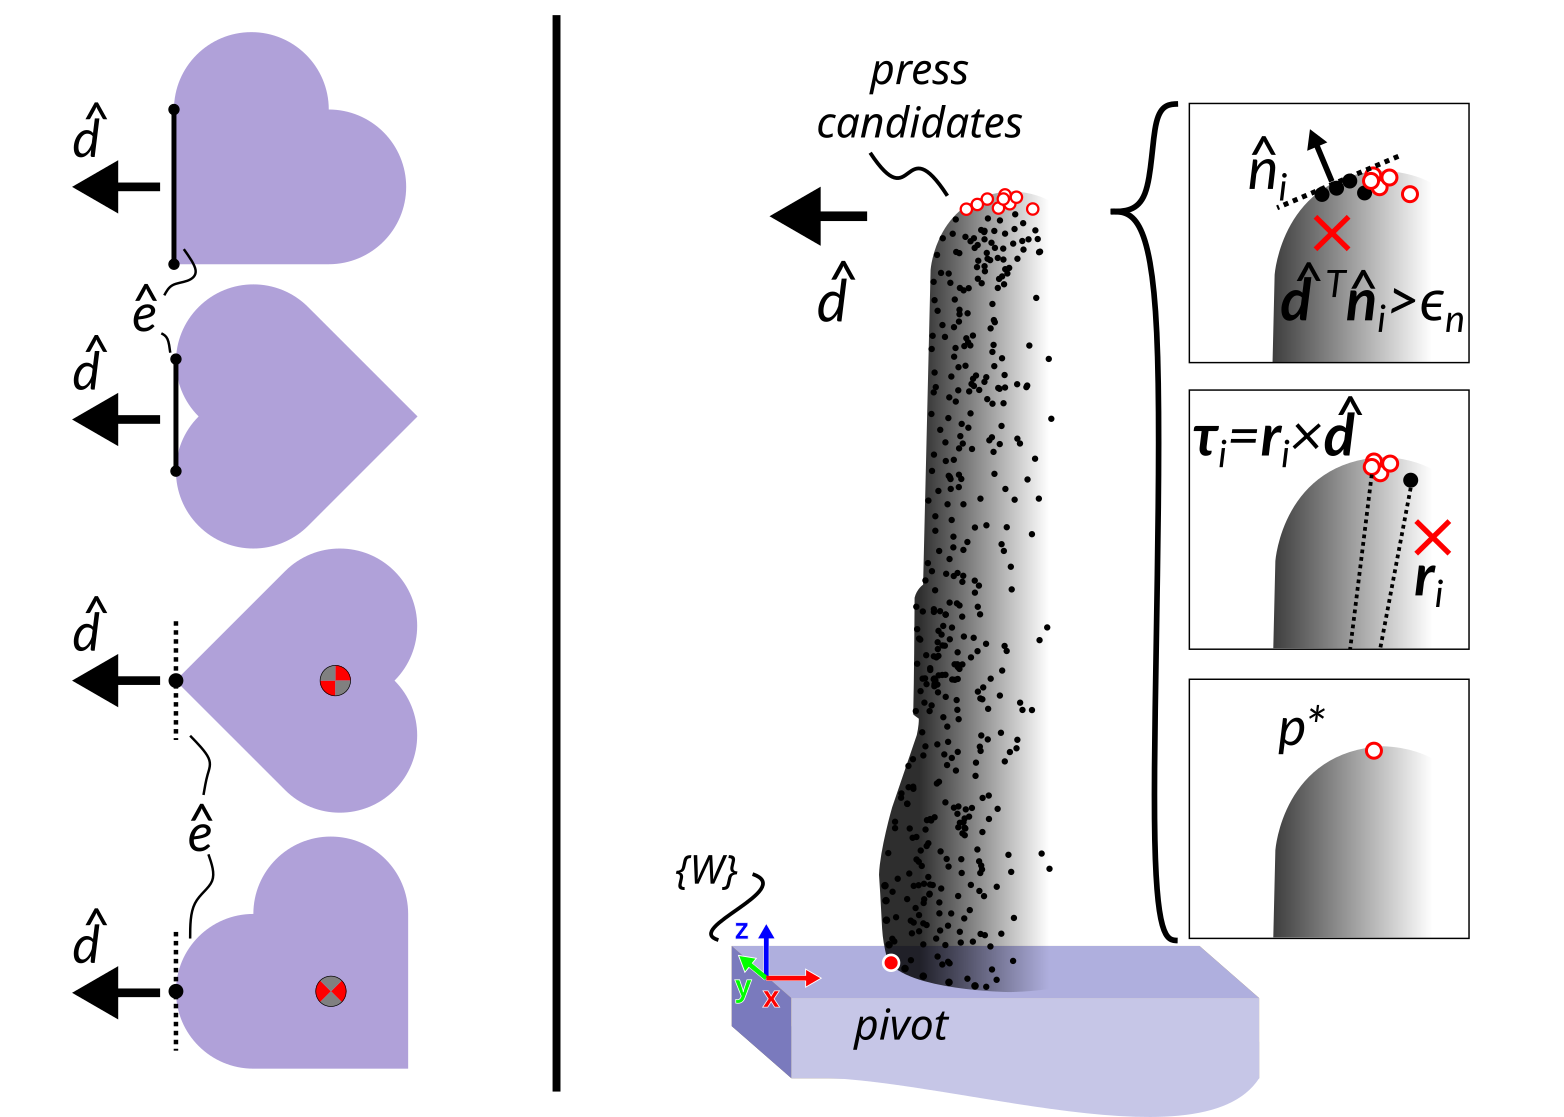
\includegraphics[width=0.95\textwidth]{figures/contact_selection.png}
  \caption{Tipping direction and press-point selection.
  (\textbf{left}) Support-footprint geometry, viewed from above, for representative pivot cases. For a straight-edge pivot, the desired tipping axis $\hat{\mathbf e}$ is aligned with the edge and the pull direction $\hat{\mathbf d}$ is chosen approximately normal to it. For a vertex or locally curved support boundary, contact reduces to a single expected pivot point and $\hat{\mathbf e}$ is taken as the local tangent to the support boundary.
  (\textbf{right}) Press-point selection on a segmented object point cloud $\mathcal{P}$, shown for the pull direction $\hat{\mathbf d} = \hat{\mathbf d}_{\mathrm{pull}}$. Candidate points are first screened by the surface-normal condition in Eq.~\eqref{eq:press_feasible_set} to reject contacts likely to separate under the commanded pull. For each remaining point, the lever arm $\mathbf r_i$ and resulting moment $\boldsymbol{\tau}_i = \mathbf r_i \times \hat{\mathbf d}$ are evaluated. The selected point $\mathbf p^*$ maximizes the signed moment about the desired tipping axis according to Eq.~\eqref{eq:press_point_selection}. Forward tipping reuses the same construction at $\hat{\mathbf d}_{\mathrm{push}}$ (Section~\ref{sec:forward_tip_selection}).}
  \label{fig:contact_selection}
\end{figure*}

% OFFICIAL AND MORE RIGOROUS VERSION PROVIDED BY CONTACT_SELECTION FIGURE. THIS ONE IS DEPRECATED.
% \begin{figure}[t]
%   \centering
%   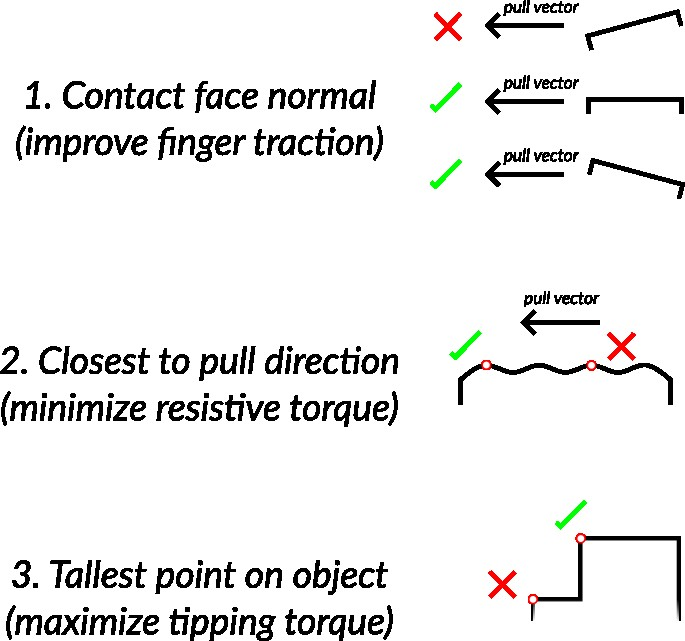
\includegraphics[width=0.85\linewidth]{figures/press-selection.jpg}
%   \caption{The three press-point preferences, in order: (1) a contact-face normal that does not lean away from the pull, to keep fingertip traction; (2) the candidate closest to the pivot along the pull direction, to minimize the resistive press torque; (3) the tallest point on the object, to maximize tipping leverage. Eq.~\eqref{eq:press_demand} trades (2) against (3) through fingertip friction. \sh{New figure; decide whether it replaces the right panel of Fig.~\ref{fig:contact_selection} or sits beside it.}}
%   \label{fig:press_selection}
% \end{figure}

The interaction direction is selected from the expected tipping geometry (Fig.~\ref{fig:contact_selection}, left). We write $\hat{\mathbf d}$ for the commanded direction in the support plane, instantiated as the pull direction $\hat{\mathbf d}_{\mathrm{pull}}$ here and as the push direction
$\hat{\mathbf d}_{\mathrm{push}}$ for forward tipping (Section~\ref{sec:forward_tip_selection}). For an object expected to rotate about a straight tipping edge with unit direction $\hat{\mathbf e}$, $\hat{\mathbf d}$ is chosen approximately normal to the edge and parallel to the support surface. For objects with a locally curved support boundary and a single expected pivot point, $\hat{\mathbf d}$ is instead chosen approximately normal to the local tangent of the support boundary at the pivot. The sign of $\hat{\mathbf d}$ is selected to induce rotation in the desired tipping direction.

Given a segmented object point cloud
\begin{equation}
    \mathcal{P} = \{\mathbf p_i\},
\end{equation}

with an estimated outward surface normal $\mathbf n_i$ associated with each point, candidate contact points are first restricted to surfaces compatible with the commanded direction (Fig.~\ref{fig:contact_selection}, right). The feasible set is defined as

\begin{equation}
    \mathcal{P}_f(\hat{\mathbf d}) =
    \left\{
    \mathbf p_i \in \mathcal{P}
    \;\middle|\;
    \hat{\mathbf d}^{T}\mathbf n_i \leq \epsilon_n
    \right\},
    \label{eq:press_feasible_set}
\end{equation}
where $\epsilon_n$ permits a small outward component while rejecting surfaces for which the commanded motion would strongly promote loss of contact. The screen depends on $\hat{\mathbf d}$ alone, so the same construction serves both interactions.

For each feasible point, let $\mathbf q$ denote a point on the expected tipping edge, or the expected pivot point for a locally curved support boundary, and define the pivot-to-contact vector
\begin{equation}
    \mathbf r_i = \mathbf p_i - \mathbf q.
\end{equation}
Assuming an applied force with fixed magnitude in direction $\hat{\mathbf d}$, the resulting moment about the pivot is proportional to
\begin{equation}
    \boldsymbol{\tau}_i
    =
    \mathbf r_i \times \hat{\mathbf d}.
    \label{eq:press_point_torque}
\end{equation}

The signed component of this moment about the desired tipping axis defines the contact score
\begin{equation}
    S_i(\hat{\mathbf d})
    =
    \hat{\mathbf e}^{T}
    \left(
    \mathbf r_i \times \hat{\mathbf d}
    \right).
    \label{eq:score}
\end{equation}
For a straight tipping edge, $\hat{\mathbf e}$ is aligned with the edge; for a locally curved support boundary, it is tangent to the boundary at the expected pivot. The sign of $\hat{\mathbf e}$ is chosen such that positive $S_i(\hat{\mathbf d})$ corresponds to the desired tipping direction.

The contact point is then selected as
\begin{equation}
    \boxed{
    \mathbf p^*(\hat{\mathbf d})
    =
    \arg\max_{\mathbf p_i \in \mathcal{P}_f(\hat{\mathbf d})}
    \hat{\mathbf e}^{T}
    \left[
    \left(
    \mathbf p_i - \mathbf q
    \right)
    \times
    \hat{\mathbf d}
    \right]
    }
    \label{eq:press_point_selection}
\end{equation}
so that press-and-pull presses at $\mathbf p^*_{\mathrm{pull}} = \mathbf p^*(\hat{\mathbf d}_{\mathrm{pull}})$, the point marked $\mathbf p^*$ in Fig.~\ref{fig:contact_selection}. This objective favors candidates with a large moment arm perpendicular to the commanded direction while penalizing points that generate moment in the opposing tipping direction. Equivalently, since $\|\boldsymbol{\tau}_i\| \propto \|\mathbf r_i\|\sin\theta_i$, where $\theta_i$ is the angle between $\mathbf r_i$ and $\hat{\mathbf d}$, high-scoring points tend to have large lever arms oriented approximately orthogonal to the commanded direction.

\subsubsection{Accounting for the press itself}
\label{sec:press_demand}
Eq.~\eqref{eq:press_point_selection} scores the pull alone. The press does two jobs at once: the added normal force keeps the object from sliding, and loading the pivot edge pins it to avoid swirling or other rotation. But a press applied inboard of the pivot also adds a moment that resists tipping. For irregular-top objects, such as the soda bottle, the highest point is very far from the pivot, and the press force fights against the tipping torque. The press point is therefore a multi-objective problem (Table~\ref{tab:press_objectives}): it should sit as close to the pivot edge (horizontally, in the pull direction) as the top surface allows, and as high on the object as possible.

\begin{table*}[t]
  \centering
  \caption{Press point selection objectives and constraints.}
  \label{tab:press_objectives}
  \small
  \begin{tabular}{p{0.16\textwidth} p{0.08\textwidth} p{0.33\textwidth} p{0.33\textwidth}}
    \toprule
    \textbf{Term} & \textbf{Role} & \textbf{Net effect / reasoning} & \textbf{When it binds or competes} \\
    \midrule
    Close to the pivot edge (horizontally) & Objective & The press adds as little torque against tipping as possible. Loading the pivot edge also pins it, so the object tips stably. & Competes with height on domed or irregular tops (flashlight, heart), where the highest point lies far from the pivot. \\
    High on the object & Objective & The pull gains as much tipping leverage as possible once it begins. & Irrelevant on a flat top: every point is at the same height, so the rule reduces to the point nearest the pivot edge. \\
    Inside the observed top surface, with margin & Constraint & The margin absorbs point-cloud error, so the fingertip does not land off the edge of the object. & Pushes the point inward from the pivot edge, most on noisy or thin tops. \\
    Reachable, collision-free approach & Constraint & The fingertip can actually get to the point. & Tall objects or cluttered workspaces. \\
    Fingertip holds without slipping & Constraint & The added normal force keeps the object from sliding only if the fingertip itself holds under the pull. & Low fingertip--top-face friction or heavy objects, where the press needed grows large (the monitor). \\
    \bottomrule
  \end{tabular}
\end{table*}

The two objectives trade off through a single quantity. Consider a locally horizontal press surface at height $H$ above the table, a downward press $P$, and a horizontal pull $T$ toward the near pivot edge. Let $d$ be the inward horizontal distance from the projected CoM to that edge and $a$ the contact's inward horizontal offset from it. Tipping begins, and neither contact slips, when
\begin{equation}
    TH \ge mgd + aP, \qquad T \le \mu_t(mg + P), \qquad T \le \mu_f P,
    \label{eq:pp_onset}
\end{equation}
where $\mu_f$ is the fingertip--top-face friction coefficient. The term $aP$ is the inboard-press penalty: increasing the press improves traction but also makes tipping harder. Normalizing by the unknown weight, $p = P/(mg)$, removes the mass that the interaction is meant to estimate:
\begin{equation}
    d + ap \le \mu_t H (1+p), \qquad d + ap \le \mu_f H p.
    \label{eq:pp_normalized}
\end{equation}
For positive $d$, fingertip traction requires $\mu_f H > a$ and
\begin{equation}
    \boxed{\, p \;\ge\; p_{\min} = \frac{d}{\mu_f H - a} \,}
    \label{eq:press_demand}
\end{equation}
intersected with the table constraint $(a - \mu_t H)\,p \le \mu_t H - d$. The minimum normalized press demand $p_{\min}$ resolves the height-versus-distance trade in closed form: height $H$ lowers the demand, the inward offset $a$ raises it, and the exchange rate between them is the fingertip friction $\mu_f$. As $a \to \mu_f H$ the required press diverges, and for $a \ge \mu_f H$ no press load is feasible: this is the monitor, whose only usable press point is far inside the support polygon. We therefore select the press point that minimizes $p_{\min}$ over the camera-validated candidates, subject to the constraints of Table~\ref{tab:press_objectives}. \sh{Decision from the outline: is minimizing $p_{\min}$ the answer to ``how height is traded against distance to the pivot on domed tops''? Implementation currently uses the torque score \eqref{eq:press_point_selection} plus the camera check; $p_{\min}$ is planned in tipping\_mode\_selector\_plan.md. Needs $d$ and a $\mu_f$ prior.} \jx{We talked about using two conditions, (1) contact normal is away from the pull direction by some angle, and (2) contact point is closer to the robot base, for optimizing the selection of the press point.} \sh{(1) is the normal screen $\epsilon_n$ in \eqref{eq:press_feasible_set}; (2) can enter as a reach tie-breaker.}

The surface-normal screen is complemented by a camera-validated top-support check: each candidate is projected into every camera, local planes are fit to its 8 and 12\,mm neighborhoods, and the candidate passes only if the fits are planar, agree in normal direction within $20^\circ$ across scales, and agree across cameras; conflicting or absent views abstain rather than pass. These thresholds are experimental, not calibrated uncertainty estimates. \sh{Report the pass/reject/uncertain counts across the campaign.}

\subsection{Forward-Tipping Contact Selection}
\label{sec:forward_tip_selection}

Forward tipping is the same selection without the press. The tipping axis $\hat{\mathbf e}$, the pivot $\mathbf q$, the lever arm $\mathbf r_i$, the feasible set \eqref{eq:press_feasible_set}, and the score \eqref{eq:score} all carry over unchanged, evaluated at $\hat{\mathbf d}_{\mathrm{push}}$, so the
push contact is
\begin{equation}
    \boxed{
    \mathbf p^*_{\mathrm{push}}
    =
    \mathbf p^*(\hat{\mathbf d}_{\mathrm{push}})
    }
    \label{eq:forward_tip_selection}
\end{equation}
The one difference is what maintains contact. The push is compressive, so contact is held by the applied force itself rather than by friction under a separate press, and no contact-maintenance criterion beyond
\eqref{eq:press_feasible_set} is required; we therefore take $\epsilon_n = 0$ for forward tipping, admitting only faces the push acts into, while press-and-pull tolerates $\epsilon_n > 0$ because the press holds contact.

For an approximately horizontal push, the same lever-arm argument favors higher contact points, recovering the conventional heuristic of pushing near the top of the object to promote tipping. The point should also be on a face whose inward normal passes near or through the planar CoM projection, and should have a corresponding ``nice'' tipping edge on the opposite side of the object, like a line pivot. The far pivot edge is observed by a fixed camera on the opposite side of the object.

\noindent \textbf{Planar push point.} The sliding push point is the lowest point the fingertip can reach freely, as in \isrr{}. We do not care if the object swirls at this moment, so pushing through the CoM planar projection is not expressly required. Only certain very tall, high-friction objects will be unable to slide and will exclusively tip.

\subsection{Interaction-Mode Selection}
\label{sec:mode_selection}

After the object has been observed and a planar push has been performed, the robot selects an initial tipping interaction. Because the object's mass, object--support friction coefficient, and force required to initiate tipping are not known a priori, the initial mode selection is based only on observable support geometry.

The expected tipping pivot is classified as either an extended edge or an isolated point. Forward tipping is selected when the support geometry provides an extended tipping edge, which constrains the instantaneous rotation axis during the interaction. When the expected pivot reduces to a single point, such as at a sharp vertex or along a locally curved support boundary, the press-pull mode is selected.

The initial interaction mode is therefore
\begin{equation}
    \boxed{
    \text{Mode}_0 =
    \begin{cases}
        \text{Press-pull}, & \text{isolated-point pivot}, \\[4pt]
        \text{Forward tip}, & \text{extended-edge pivot}.
    \end{cases}
    }
    \label{eq:mode_selection}
\end{equation}

The planar sliding force measured before tipping is retained for subsequent physical-property estimation, but is not used to determine the initial tipping mode because it reflects the combined effect of unknown mass and friction. Information obtained during the first tipping interaction may be used to adapt a second interaction in response to observed sliding or pivot instability. \sh{The paragraphs above describe the interim geometric rule (implemented 2026-10-13). The three-step heuristic below extends it; merge the two once the selector is final.}

\noindent \textbf{Two modes, two purposes.} The two modes are not a main method and a fallback; they serve different purposes. Press-and-pull is for objects that would slide or tip unstably on their own, since the press prevents the sliding and pins the pivot. Forward tipping is for objects that press-and-pull suits poorly: those with a poor top contact, and those heavy enough that the fingertip cannot hold the pull without slipping. The monitor is the clearest example; it needed a large press just to keep the fingertip from slipping, but tips very readily otherwise. Where both would work, we choose forward tipping for its simplicity, unless instability is predicted or observed. The robot decides in three steps (Fig.~\ref{fig:flowchart}):

\noindent \textbf{Step 1, predict instability from base roundness.} Judged from the point cloud prior to contact. A rounded base lets the pivot roll and the object swirl; in \iros{}, the flashlight swirled late in the tip. The forward pivot is fit from the far camera's segmentation and classified as straight (a sharp line contact) or curved (otherwise), following JX's definition: an edge is sharp with a line contact; otherwise, it is round. A base more round than a threshold is sent to press-and-pull. The threshold comes from the fillet sweep (Section~\ref{sec:results}). \sh{What measure of roundness? How large of a base radius is an ``edge'' rather than ``round''? Consider a water bottle vs.\ a trash can. Currently a chord-straightness test on the cam3 SAM fit; a $\sim$25\,mm chord of cylinder\_e can still pass as straight.}

\noindent \textbf{Step 2, catch sliding before it happens.} For a horizontal push at contact height $h$ with horizontal lever $L$ from the pivot, the push force needed to start tipping and the force at which the object starts to slide are
\begin{equation}
    N_{\mathrm{tip}} = \frac{mgd}{h - \mu_f L}, \qquad N_{\mathrm{slide}} = \frac{\mu_t m g}{1 - \mu_t \mu_f},
\end{equation}
and their ratio, the \emph{competition of sliding and tipping},
\begin{equation}
    \boxed{\, \mathrm{CoST} = \frac{N_{\mathrm{slide}}}{N_{\mathrm{tip}}} = \frac{\mu_t (h - \mu_f L)}{d\,(1 - \mu_t \mu_f)} \,}
    \label{eq:cost}
\end{equation}
contains neither the mass nor the CoM height, so it can gate the choice before anything is estimated. Forward tipping is preferred when $\mathrm{CoST} > 1 + \epsilon$; the margin $\epsilon$ is a heuristic preference, not a guarantee. This prediction is verified in contact by a \emph{slide probe}: at 10\,mm of push travel the finger backs off 2\,mm; a tilted object rests on its edge and follows the finger back under gravity, keeping at least 30\% of its force, while one that slid stays put and the force vanishes. A detected slide sends the object to press-and-pull, and the slide itself is kept as a friction sample, since for a horizontal push that same force is the most a forward-tipping push can apply before the object slides. \sh{Verify the $\mu_f L$ term and sign convention of \eqref{eq:cost} against the derivation in vision\_vs\_proprioception\_results.md \S7. Decide: after a slide probe, abort (current) or re-probe until a slide budget runs out, which keeps slide-then-tip runs like tipT\_a?}

\noindent \textbf{Step 3, check that press-and-pull is usable.} The most important factor is whether the press point is near the pivot. For objects where the only press point is far inside the support polygon, the press generates a large moment that resists tipping, and the normalized demand $p_{\min}$ of \eqref{eq:press_demand} grows without bound. Selecting a lower press point is not always feasible, and too low would require a very large pull force. Press-and-pull is admitted only when the feasible interval of \eqref{eq:pp_normalized} is non-empty and $p_{\min}$ lies inside an empirically supported envelope. If neither mode qualifies, the robot reports an unsupported object rather than forcing a mode. \sh{The $p_{\min}$ envelope must be calibrated on development data and labeled as such; it does not establish actuator feasibility in newtons without mass.}

\noindent \textbf{Recovery when the choice does not hold up.} Each attempt ends with a classified outcome, and a bounded cascade chooses the next attempt from \emph{why} the previous one failed (Table~\ref{tab:cascade}). Press-and-pull starts at the contact closest to the pivot, where a harder press costs nothing in tipping moment, so on fingertip slip more force is the cheapest fix and comes before a riskier contact. The cascade is capped at four attempts in total, takes a fresh snapshot after every attempt, never exceeds 13\,N of press, and stops at the first sign the object moved or fell. A slide that leaves the object upright is not counted as ``moved''; the next attempt runs on the new snapshot.

\begin{table*}[t]
  \centering
  \caption{Failure $\rightarrow$ next attempt. Every outcome is detected from signals already logged by the controllers.}
  \label{tab:cascade}
  \small
  \begin{tabular}{p{0.10\textwidth} p{0.22\textwidth} p{0.32\textwidth} p{0.26\textwidth}}
    \toprule
    \textbf{Mode} & \textbf{What happened} & \textbf{How we see it} & \textbf{Next try} \\
    \midrule
    Press-pull & Fingertip slipped on top & Lost contact ($<0.3$\,N for 20 samples) or ball-to-pivot spread $>4$\,mm & More force ($\times1.25$, up to 13\,N) $\rightarrow$ higher candidate $\rightarrow$ forward tip \\
    Press-pull & Arc limit reached before balance, no slip & No pull-force sign flip by the arc limit & Counted as success; optionally higher candidate or larger arc \\
    Press-pull & Object slid on the table & Pivot fitted from the ball's arc moves, or before/after snapshots shifted & More force $\rightarrow$ stop \\
    Forward & Hit the force limit & Axial force $>20$\,N & Press-and-pull \\
    Forward & Finger drifted off the face & Height, lateral, or orientation drift & Press-and-pull \\
    Forward & Slid instead of tipping & Slide probe: force vanishes on the 2\,mm back-off & Keep as friction sample; press-and-pull \\
    Forward & Too easy: nearly toppled & Force fails to reach 0.30\,N within 1.5\,mm of touch & Back off; press-and-pull (holds the object through balance about the other edge) \\
    Either & Missed contact, bad geometry & Below predicted contact height; planning failure & New snapshot, retry once $\rightarrow$ next candidate \\
    Either & Sensor fault & Stale or non-finite wrench, stale pose & Retry the same step, no escalation \\
    Either & Object moved, rotated, or fell & Before/after snapshot difference & Stop and report \\
    \bottomrule
  \end{tabular}
\end{table*}

\noindent \textbf{A challenging object.} The hard case is a light object that prefers to slide and has a poor top contact. It slides, so forward tipping reaches the sliding limit before it tips and the heuristic sends it to press-and-pull. Its top contact is poor, so press-and-pull is also a bad fit. And being light, it produces a small gravitational torque, so the signal being measured is weak against the applied forces. We name this case up front, predict it from \eqref{eq:press_demand}--\eqref{eq:cost}, and demonstrate the pipeline on it: it is better to show a predicted worst case than to explain it after the fact. \sh{Which object? Candidates: soda bottle (domed top), the 3D-printed bottle, or the pen cup. Write the prediction before running.} \jx{If an object has the CoM close to the top but a large base for stability on the table, will it be difficult to slide or tip it?}

%% ==============================================
\section{One Estimator for Both Modes} \label{sec:estimation}
%% ==============================================

Both primitives rotate a rigid object about a known pivot edge while the wrist force/torque sensor reads the finger wrench, so both are served by one estimator. The primitives differ only in \emph{where the object tilt $\varphi(t)$ comes from}, so tilt is treated as a pluggable input; everything else (rocking-onset detection, torque about the pivot, fitting the push and return branches, and tip/slide labeling) is computed once. Routing the press-and-pull data of \isrr{} through the shared estimator reproduces the earlier results bit for bit across 47 trials (largest difference $10^{-16}$).

\subsection{What a single tip can identify} \label{sec:identifiability}

For rotation about a straight pivot edge, the gravity torque about the edge depends only on the CoM's horizontal distance \emph{perpendicular to the edge}, the in-board distance $d$, and its height $z_c$ above the pivot. With vertical gravity and absolute tilt $\varphi$,
\begin{equation}
    \tau(\varphi) = g\,\big[(m d)\cos\varphi - (m z_c)\sin\varphi\big] = mg\,r\sin(\theta^{*} - \varphi),
    \label{eq:tau_model}
\end{equation}
with $r = \sqrt{d^2 + z_c^2}$ and $\tan\theta^{*} = d/z_c$. The CoM's position \emph{along} the edge does not enter; it only needs to lie within the edge's extent so the object rocks on the edge instead of rolling off a corner. The torque curve is invariant under
\begin{equation}
    (m,\ d,\ z_c) \;\to\; (\lambda m,\ d/\lambda,\ z_c/\lambda),
    \label{eq:lambda_invariance}
\end{equation}
so a single pivot identifies only the mass-weighted first moments $m d$ and $m z_c$, equivalently $m r$ and $\theta^{*}$. This is the same base-parameter structure known from payload identification \cite{atkeson_rigid_1985}, except that here the pivot reaction hides the gravity \emph{force}, so even $m$ is lost and only the moment survives. No additional fitting freedom escapes \eqref{eq:lambda_invariance}; breaking it needs extra physics or data. Tipping about several supports does so, which is the equi-effect approach of \cite{yong_yu_estimation_1999}; we instead take the planar CoM, and therefore $d$, as a known input from prior pushing \cite{hyland_predicting_2023}, report $m$ and $z_c$ conditional on it, and report $m r$ and $\theta^{*}$ alongside as the $d$-independent check. Choosing the CoM as the frame origin does not help: it removes the gravity moment from the balance but introduces the same unknown support geometry through the table-reaction moment. \sh{Reviewer-facing: keep the dual-tip discussion to one sentence (``considered, not pursued, since it is the prior literature's approach'').}

\subsection{Estimation methods}
All methods fit pivot torque against tilt on the push (tip) and return branches separately and average the two.
\begin{itemize}
  \item \textbf{Method A, zero crossing.} Extrapolate $\tau(\varphi)$ to zero to obtain $\theta^{*}$, then $z_c = d/\tan\theta^{*}$.
  \item \textbf{Method B, free fit with absolute tilt.} Fit $m$ and $z_c$ in \eqref{eq:tau_model} with $\varphi$ taken exactly as measured. A tilt-zero error $\delta$ shifts $\theta^{*}$ by $\delta$, so $\delta z_c/z_c = -\delta/(\sin\theta^{*}\cos\theta^{*})$: 5.5--7.6\% per degree for the Tip-T configurations and about 20\% for a tall object with $\theta^{*} = 5^\circ$. The residual does not show it.
  \item \textbf{Method D, anchored at rocking onset (primary).} At onset the object is upright, so $\tau_{\mathrm{on}} = m g d$ gives $m$ without any tilt measurement. With $m$ fixed, fit $z_c$ and a constant tilt offset $\varphi_0$. Only tilt increments matter, so a slide before rocking or a wrong tilt zero does not bias the result; $\varphi_0$ should come out near zero.
\end{itemize}
Methods B and D describe the same two-coefficient sinusoid and have identical residuals; D merely assigns $m$ from the onset torque. Their agreement in fit quality is therefore not independent confirmation of the mass. \sh{Freeze the onset definition before the campaign: the bias audit found that an extra 25-sample moving average on the onset torque lowers mass by 1--2\%, and that the selected peak can be after true lift (Section~\ref{sec:prelim}).}

\subsection{Vision for the mode, touch for the amount}
\noindent \textbf{Proprioceptive tilt.} Finger pose plus a contact model: the finger locked to the object (press-and-pull) or a ball sliding on a planar face (forward tip). Accurate and 100\,Hz, but it assumes a contact mode, so it cannot tell tipping from sliding: the finger trajectory is consistent with either.

\noindent \textbf{Vision tilt.} Each frame from the side camera is fit for object tilt about the pivot plus slide along the push, using depth and calibration from the pre-tip perception with the finger masked out. It measures the object itself, so it separates tip from slide and gives the slide distance, but at about 30\,Hz with lower signal-to-noise. Video-to-log synchronization is fit from the tracked finger ball.

We therefore use vision to identify the contact mode and proprioception to measure tilt within it. The split follows what each sensor can actually observe, and the two tasks have very different margins: classification separates 35\,mm of slide from 0\,mm, or $13^\circ$ of tilt from $1^\circ$, so coarse sensing is enough, whereas $z_c = d/\tan\theta^{*}$ sits at a sensitive operating point. Method D is designed to absorb a tilt \emph{offset}; vision's dominant error is a tilt \emph{scale} error, which D cannot absorb, since with $m$ fixed $\hat z_c \approx k z_c$ for a scale factor $k$. Because vision is independent of the contact model, agreement between the two sources also tests that model. This is a hybrid-estimation structure, identifying the discrete contact mode first and the continuous parameters given that mode; accuracy is conditional on the label, which argues for a confidence score and an abstain option. In the caption and talk version: \emph{the camera tells us what happened; touch tells us how much.}

\subsection{Friction}
Friction follows from slides: the planar push gives the breakaway force $\mu_s m g$ and the steady sliding force $\mu_k m g$, and dividing by the tip's $m$ gives $\mu_t$. Forward tips that the slide probe labels as slides, and slides before a successful tip (tipT\_a slid 35\,mm and then tipped), are kept as additional friction samples; probe samples themselves are a separate branch and are never fitted.

\subsection{An observability gate that needs no prior}
As $d \to 0$ the gravitational moment $mgd$ drops into the sensor noise, and three things fail together: contact detection, the onset-torque mass of method D ($\tau_{\mathrm{on}} = mgd \rightarrow 0$), and stability ($\theta^{*} \rightarrow 0$, so the object topples with a nudge). The forward-tip controller requires the force to reach 0.30\,N within 1.5\,mm of touch (touch itself is declared at 0.05\,N); otherwise it backs off as \emph{too easy}. For the Tip-T this is equivalent to $\tau_{\mathrm{on}} \gtrsim 0.047$\,N\,m, or $d \gtrsim 12$\,mm at 0.404\,kg. It gates exactly the onset torque that method D uses, with no mass or CoM prior, and so it remains valid when the known $d$ is slightly wrong.

%% ==============================================
\section{Keeping the Interaction Safe} \label{sec:method}
%% ==============================================

\begin{figure}[t]
  \centering
  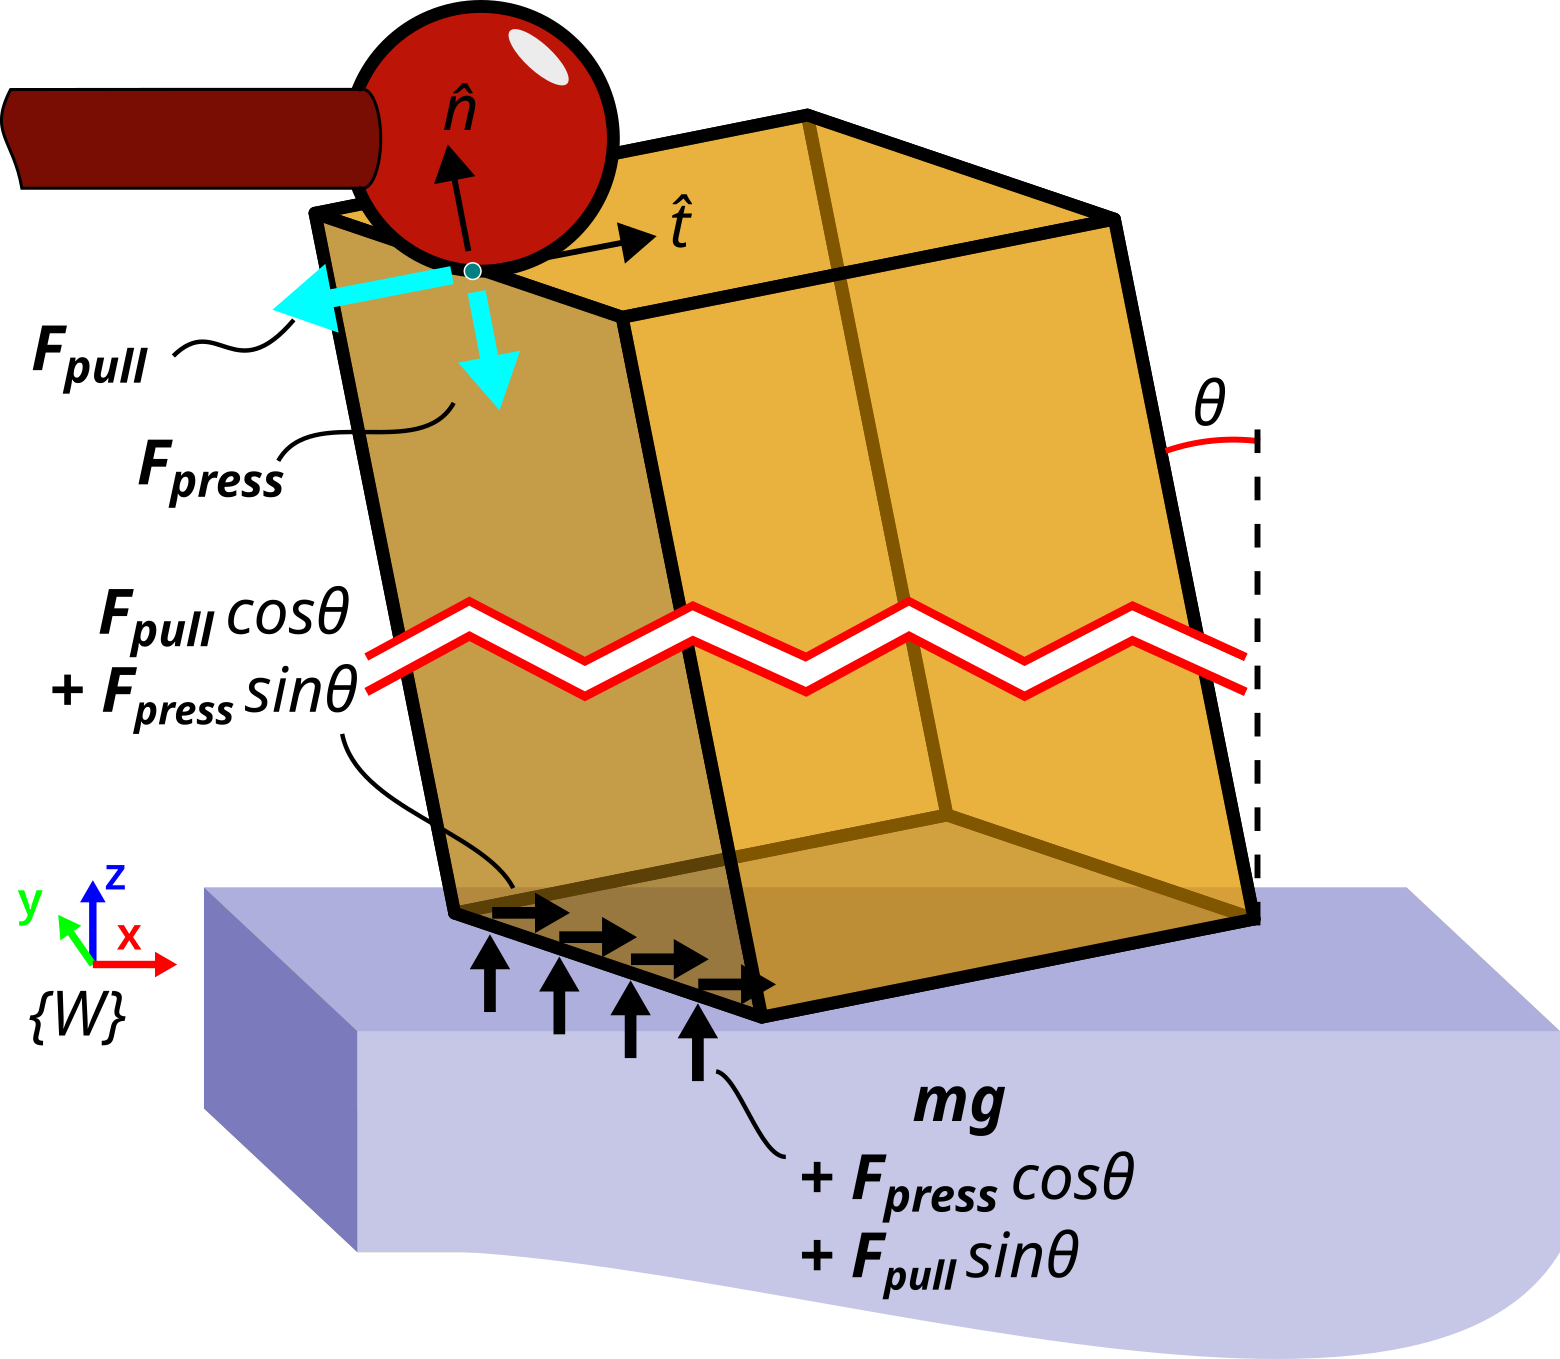
\includegraphics[width=0.95\linewidth]{figures/zoom.png}
  \caption{Normal and tangential balances at the table contact during press-and-pull. As $\theta$ grows, the maintained press acquires a world-horizontal component $F_{\mathrm{press}}\sin\theta$ that adds to the tangential load. \sh{Show the friction cone in this figure?}}
  \label{fig:zoom}
\end{figure}

The estimation interaction must drive the object far enough up the tipping arc to observe the parameters cleanly, without letting either of its contacts slip. For press-and-pull, we show why toppling is a consequence of slip rather than an independent hazard, derive the coupling between the press and the table-slip constraint, and define a single margin over the whole arc. For forward tipping, we state the stopping rule and why only press-and-pull can cross the balance point safely. \textbf{Notation.} The ISRR and IROS papers use $\eta_{\mathrm{safety}}$ for the threshold at which the tip stops, defined as a fraction of the peak pull (or push) force; we keep that meaning, and name the new slip margin $\eta_{\mathrm{slip}}$.

\subsection{Problem setup}
We analyze the tipping motion in the vertical plane containing the pull direction and the pivot, parameterized by the object angle $\theta \in [0, \theta_{\mathrm{end}}]$, where $\theta_{\mathrm{end}}$ is set by the slip margin rather than fixed a priori. $\theta^{*}$ denotes the \emph{toppling angle} at which the CoM passes over the pivot; it is a waypoint the arc may or may not cross, not a boundary on $\theta_{\mathrm{end}}$. The press force is maintained along the object's top-face normal $\hat{\mathbf{n}}(\theta)$ throughout the motion. Observing Figure~\ref{fig:zoom}, control is applied in this finger-fixed frame: $F_{\mathrm{press}}$ is a regulated normal force held throughout the arc, while the pull is a velocity command along $\hat{\mathbf{t}}(\theta)$ and $F_{\mathrm{pull}}(\theta)$ denotes the resulting signed tangential component. Because the pull is kinematic, $F_{\mathrm{pull}}$ reverses sign on its own as the object crosses $\theta^{*}$; no force-switching logic is needed and the equations hold unchanged across the crossing. The object--table contact supports a normal force $N_t(\theta)$ and a tangential reaction $f_t(\theta)$ that must remain within the friction cone.

\subsection{Two contacts, one governing hazard}
The press-and-pull primitive maintains two passive-grasp contacts throughout the arc: the finger against the object's top face, and the object's base against the table. As long as neither contact slips, the object is kinematically locked to the commanded pivot rotation and cannot fall over on its own. An uncontrolled topple is only possible if one of these constraints is broken by a slip. Toppling is therefore only a consequence of a prior slip, and bounding the friction-cone margin at both contacts is sufficient to prevent it.

We hold the finger--object contact by design with a rigid, high-friction fingertip pressed with sufficient force, verified after the fact by the ball-to-pivot spread and by lost-contact detection (Table~\ref{tab:cascade}). The hazard we certify is how close the table contact is to slipping (the \emph{slip margin}); we additionally track proximity to the toppling angle (the \emph{toppling margin}) as a diagnostic, not as a second constraint. The monitor is the observed exception: its fingertip slipped during press-and-pull (an 8.4\,mm ball-to-pivot spread against a 4\,mm tolerance), which is why the mode heuristic sends it to forward tipping.

\noindent \textbf{Toppling.} At $\theta^{*}$ the gravitational moment about the pivot changes sign: below it, gravity restores the object and sustaining quasistatic rotation requires an outward pull; beyond it, gravity itself continues the rotation, so sustaining a controlled increase in $\theta$ requires the applied load to reverse into a hold-back force. Because the object remains locked to the arc as long as neither contact slips, this sign flip is not itself a fall; it is safe for as long as the reversed load stays inside the table-slip margin. We track it with the toppling margin
\begin{equation}
    \lambda_{\mathrm{topple}}(\theta) = \frac{F_{\mathrm{pull}}^{\mathrm{meas}}(\theta)}{F_{\mathrm{pull}}^{\mathrm{peak}}}
    \;\in\;(-\infty,1],
    \label{eq:m_topple}
\end{equation}
which is near $1$ early in the arc, crosses zero exactly at $\theta^{*}$, and continues negative beyond it. Here $F_{\mathrm{pull}}^{\mathrm{peak}} \triangleq F_{\mathrm{pull}}(\theta \to 0)$, fixed at the onset of the pull so that $\lambda_{\mathrm{topple}}$ is evaluable from the first instants of interaction. Whether an arc can cross $\theta^{*}$ is decided entirely by the slip margin. Crossing is preferred when available: it replaces an asymptotic extrapolation with a direct zero-crossing observation, sharpening $z_c$.

\noindent \textbf{Object--table slippage.} The table contact slips when $\lVert f_t(\theta)\rVert = \mu_t N_t(\theta)$, where the dominant contributions are
\begin{align}
    N_t(\theta) &\approx mg + F_{\mathrm{press}}\cos\theta + F_{\mathrm{pull}}(\theta)\sin\theta, \label{eq:Nt}\\
    \lVert f_t(\theta)\rVert &\approx F_{\mathrm{pull}}(\theta)\cos\theta + F_{\mathrm{press}}\sin\theta,
    \label{eq:ft}
\end{align}
the projections of the maintained press and pull onto the world vertical and horizontal as the press-face normal rotates with $\theta$. The $\approx$ neglects second-order terms from the finite contact patch at the pivot. The corresponding slip margin is the normalized friction-cone slack,
\begin{equation}
    \lambda_{\mathrm{slip}}(\theta)
    = 1 - \frac{\lVert f_t(\theta)\rVert}{\mu_t\, N_t(\theta)}
    \;\in\;(-\infty, 1],
    \label{eq:m_slip}
\end{equation}
positive inside the cone and zero at incipient slip.

\subsection{The coupling and the safe press band}
Equations \eqref{eq:Nt}--\eqref{eq:ft} expose the central structural fact of press-and-pull: the press force enters both the normal and tangential balances, with opposite effect on the slip margin as $\theta$ grows. Early in the arc, raising $F_{\mathrm{press}}$ raises $N_t$ and improves $\lambda_{\mathrm{slip}}$; a sufficiently large press is what makes the object tip rather than slide at all. Late in the arc, the $F_{\mathrm{press}}\sin\theta$ term inflates the tangential load faster than $\cos\theta$ sustains the normal force, so the \emph{same} press now erodes $\lambda_{\mathrm{slip}}$. A larger press is therefore not uniformly safer. For a given object there is a bounded safe press band
\begin{equation}
    \mathcal{F}_{\mathrm{press}} = \left[\, \underline{F},\; \overline{F} \,\right]:
    \quad \underbrace{F_{\mathrm{tip}} < \mu_t (mg + \underline{F})}_{\text{tipping feasible}}, \quad \underbrace{\lambda_{\mathrm{slip}}(\theta) \geq 0 \;\; \forall \theta \;\text{at}\; \overline{F}}_{\text{no late-arc slip}}
    \label{eq:press_band}
\end{equation}
whose lower bound is set by tipping feasibility and whose upper bound is set by late-arc slip. The adaptive press loop of \isrr{} searched for \emph{a} point inside $\mathcal{F}_{\mathrm{press}}$ by retrying, increasing the press only after a completed failed arc. The band's limits depend on the very $(m, \mu_t)$ being estimated, but once the slide has measured $\mu_t m g$ and $m$ settles early in the pull, the margin trajectory for the remainder of the arc follows from \eqref{eq:Nt}--\eqref{eq:ft}. The lower bound is the dimensional counterpart of the normalized press demand \eqref{eq:press_demand}. \sh{The band generalizes to a press schedule $F_{\mathrm{press}}(\theta)$ (a ``tube''); keep that as one sentence and future work unless we run it. We keep $F_{\mathrm{press}}$ constant for estimation, except where a constant press is not enough for good accuracy.}

\subsection{Admissible interaction set and slip margin}
An interaction is specified by a press force $F_{\mathrm{press}}$ and an arc ending at $\theta_{\mathrm{end}}$, which is not constrained to lie below $\theta^{*}$. A single scalar reports its worst-case proximity to the table-slip hazard over the whole arc:
\begin{equation}
    \eta_{\mathrm{slip}}
    = \min_{\theta \in [0,\theta_{\mathrm{end}}]} \lambda_{\mathrm{slip}}(\theta).
    \label{eq:eta}
\end{equation}
An interaction is admissible iff $\eta_{\mathrm{slip}} \ge \Delta_{\mathrm{slip}}$ for a prescribed buffer $\Delta_{\mathrm{slip}} \in (0,1)$, and the admissible set $\mathcal{A} = \{ (F_{\mathrm{press}}, \theta_{\mathrm{end}}) : \eta_{\mathrm{slip}} \ge \Delta_{\mathrm{slip}} \}$ collects the certified designs. The fixed sub-critical stopping rule of prior work, halting when the pull falls to a fraction $\eta_{\mathrm{safety}}$ of its peak, is recovered here as one conservative choice of $\theta_{\mathrm{end}}$ that never approaches $\theta^{*}$; fixing $\theta_{\mathrm{end}}$ that way is not required by safety, only by the older primitive's inability to reverse its own applied load. In the current implementation the arc ends at a fixed limit ($23^\circ$) or at the pull-force sign flip; reaching the limit without the flip counts as success.

\noindent \textbf{Margin traces.} Every quantity in \eqref{eq:m_slip} is available from the measured wrench \eqref{eq:adjoint}, proprioceptive $\theta$, and $\mu_t$ from the slide, so we compute $\lambda_{\mathrm{slip}}(\theta)$ along every press-and-pull trial and compare its minimum to the observed slips and retries of the reactive scheme. \sh{Decision: online predictive detector (project $\lambda_{\mathrm{slip}}$ over the remaining arc once $m$ settles, and retract before breach) vs.\ offline margin traces only. Online is not implemented; offline traces fit the two-week plan. Pose deviation from the commanded arc gives an independent geometric slip check either way.}

\subsection{Forward tipping: stopping rule and why it cannot cross}
Forward tipping holds the object only by a compressive push. Past $\theta^{*}$ the required push changes sign and a push cannot pull back, so the object falls. Forward tipping must therefore stop before balance: the controller pushes normal to the edge at constant height, arms after stable contact and 2\,mm of travel, and reverses when the axial force falls to $\eta_{\mathrm{safety}} = 10\%$ of its peak for five fresh samples, then returns along the same line to the pre-tip pose while gravity restores the object. The slide probe and the too-easy gate (Section~\ref{sec:estimation}) guard the two other ways a forward tip goes wrong, and travel, time, and force are bounded (20\,N). Only press-and-pull, which holds the object through balance between two contacts, can cross $\theta^{*}$ safely.

\subsection{Safety--accuracy tradeoff}
The same proximity that creates risk creates information, and the risk is singular: it is the slip buffer $\Delta_{\mathrm{slip}}$, not a separate toppling buffer, that trades against accuracy. The CoM height is most sharply fixed by directly observing the sign flip of $F_{\mathrm{pull}}(\theta)$ at $\theta^{*}$; whether an arc's slip budget extends far enough to cross depends on the object ($\mu_t$, mass, chosen press). A generous buffer stops short of $\theta^{*}$ for low-friction or heavily pressed objects, leaving $z_c$ to be inferred from the pre-crossing trend alone; a tighter buffer, or a more favorable press, admits the crossing and its sharper $z_c$, at reduced margin against the one hazard that remains. The mass, observable throughout the arc, is comparatively insensitive to this choice. For forward tipping the analogous knob is $\eta_{\mathrm{safety}}$. We characterize both empirically in Section~\ref{sec:results}.

\subsection{Estimation conditioning and the press band} \label{sec:conditioning}
Beyond tipping feasibility below and slip safety above, a third consideration favors the low end of the press band \eqref{eq:press_band}: estimation conditioning. Fitting $m$ relies on the gravitational moment about the pivot, whose signal-to-noise ratio scales with $m d$, so light objects and objects with $d \to 0$ are hardest. A large press worsens this: since $F_{\mathrm{press}}$ acts through the finger contact rather than the pivot, any lever-arm error injects a spurious moment (that error times $F_{\mathrm{press}}$) onto the same balance, and under a large press it can dominate the pull-torque signal and correlate the recovered $m$ with press magnitude. We therefore bias the press low during the estimation window.

\subsection{Covariance-coupled margin}
\sh{What I'm thinking for this section: inflate the buffer $\Delta_{\mathrm{slip}}$ in proportion to the estimation uncertainty, so the interaction backs off when $\mu_t, m$ are poorly estimated ($\Delta_{\mathrm{slip}} \leftarrow \Delta_{\mathrm{slip}} + \kappa\,g(\Sigma)$); the same uncertainty feeds the shove-side gate in Section~\ref{sec:validation}, ``one principle applied twice.'' Open question: (a) drop it, (b) keep it as a one-line future-work mention, or (c) run the experiment to back it? Note: the least-squares covariance is overconfident here (autocorrelated residuals, and the dominant errors are invisible in the residual), so $\Sigma$ should come from the uncertainty budget of Section~\ref{sec:uncertainty}, not the fit.}

%% ==============================================
\section{Uncertainty: From Measurements to Estimates} \label{sec:uncertainty}
%% ==============================================

The aim is to replace ``the estimator seems accurate'' with a predicted error bar per parameter, checked against ground truth. \jx{Nonlinear least squares?} \sh{Yes for method B; method D is onset-anchored plus a two-parameter least-squares fit. Say so explicitly.}

\noindent \textbf{Input error sources.} For every input we separate bias, scale, noise, and latency (Table~\ref{tab:error_sources}).

\begin{table*}[t]
  \centering
  \caption{Input error sources, their models, and how each is obtained. Values from the 2026-10-09 hardware checks and the 2026-10-15/16 forward-tip audit.}
  \label{tab:error_sources}
  \small
  \begin{tabular}{p{0.17\textwidth} p{0.30\textwidth} p{0.45\textwidth}}
    \toprule
    \textbf{Input} & \textbf{Error model} & \textbf{How obtained / current value} \\
    \midrule
    F/T wrench & Tare bias, noise, drift, gain & Static calibration over 4 poses (condition number 4.1, force residuals $\le0.075$\,N, torque $\le1.1$\,mN\,m); per-trial tare; offsets at press onset 0.026--0.081\,N; gain \sh{known-weight check pending} \\
    Tilt, proprioceptive & Offset $\delta_0$, scale $k$, noise & Contact model; offset absorbed by method D; scale checked against vision \\
    Tilt, vision & Offset, scale, noise, sync lag & Scale error 3--20\% relative to proprioception; sync offsets $<0.5$\,s \\
    Pivot location & Perception error & Independent push/return (ARC/UNARC) pivot fits: $-1.7$ to $+0.8$\,mm except the monitor \\
    Planar CoM $d$ & Measurement $\sigma$ & Prior measurement; $\delta m/m = -\delta d/d$, $\delta z_c/z_c = \delta d/d$ \\
    Onset detection & Index jitter, late zero & Side camera tilt at the selected torque peak: up to $0.5^\circ$ \\
    Gravity direction & Tilt of $\mathbf g$ in the tipping plane & Calibration suggests $0.33^\circ$ in-plane; $\approx2.8$\,mN\,m on the Tip-T if physical \sh{unverified} \\
    \bottomrule
  \end{tabular}
\end{table*}

\noindent \textbf{Propagation.} Three complementary routes. (i) Analytic, first order, which reveals the physics: $\delta z_c/z_c = -\delta\theta^{*}/(\sin\theta^{*}\cos\theta^{*})$ for a tilt offset in method B; $\hat z_c \approx k z_c$ for a tilt scale error in method D; and $\delta z_c/z_c = \delta d/d$, $\delta m/m = \delta\tau_{\mathrm{on}}/\tau_{\mathrm{on}} - \delta d/d$ in method D; overall $\Sigma_{\mathrm{out}} = J\Sigma_{\mathrm{in}}J^\top$. (ii) Full-pipeline perturbation, one input at a time at $\pm1\sigma$, combined in quadrature, as already done for press-and-pull and extended to forward tipping and vision tilt. (iii) Monte Carlo, sampling all input errors jointly including correlations, rerunning the estimator, and reporting distributions of $m$, $z_c$, and $\theta^{*}$. We do not report the least-squares covariance $(J^\top J)^{-1}\sigma^2$ as the error bar: 100\,Hz residuals are autocorrelated and the dominant errors (tilt offset, scale, $d$) are invisible in the residual.

\noindent \textbf{Validation of the budget.} With repeated trials per configuration we check coverage: does $|\hat\cdot - \mathrm{GT}|$ fall within $2\sigma_{\mathrm{pred}}$ at the right rate, and does the predicted $\sigma$ match the across-trial spread? \sh{Needs the $\times5$ repeats.}

\noindent \textbf{Sensitivity map.} We plot predicted $\sigma(z_c)/z_c$ and $\sigma(m)/m$ over $(d, z_c)$, equivalently over $\theta^{*}$ and $d$. The map shows where the method is precise, where it degrades (tall objects with small $\theta^{*}$: one degree of tilt is 20\% of $z_c$), and where it breaks ($d \to 0$). This one figure ties the edge cases, the selector thresholds, and the error bars together. \sh{Figure to make.}

%% ==============================================
\section{Experiments, Results, and Discussion} \label{sec:results}
%% ==============================================

\subsection{Experimental setup}
We use the hardware of \isrr{}: an ABB IRB120 industrial manipulator under externally guided motion (EGM), a wrist-mounted ATI six-axis force/torque sensor (SI-130-10 calibration) sampled at about 470\,Hz, fixed Intel RealSense depth cameras for object point clouds (one observing the far pivot edge and one viewing the push from the side), and a rigid finger with a high-friction rubber ball (radius 13.25\,mm) providing point contact for both modes. Perception segments the object by DBSCAN clustering and SAM masks, fuses the three views, and takes a fresh snapshot before and after every interaction. \sh{Verify camera models/count, and F/T model (Gamma?).}

\subsection{Objects}
ISRR used four objects. A journal reviewer will expect something closer to ten to fifteen, and the designed series supply many of them at once (Fig.~\ref{fig:lineup}).
\begin{itemize}
  \item \textbf{Designed, with exact ground truth.} The CoM series (Tip-T, one exterior with five internal slug placements), the base fillet series (cylinder, $R = 0$ to 30\,mm), the pivot-geometry series (heart, point and edge contacts), and the base-friction series: same geometry and mass, different bottom material. \sh{Friction materials: felt, bare PLA, PTFE tape, rubber sheet? Weigh after adding.}
  \item \textbf{Everyday, with measured ground truth.} The original objects carried forward for continuity, plus new items that ideally are difficult to grasp: the monitor (large, heavy, asymmetric), flashlight (light, round base, round top), drill (odd geometry, non-convex), toy robot model (articulated, odd geometry), pen cup, 3D-printed bottle, and tripod. \jx{Almost rigid objects. Larger objects of the size comparable to or even bigger than a monitor are very interesting because they are too large to grasp. A desktop printer? toaster?} \sh{Decide: printer or toaster; articulated toy model and tripod conflict with the stated exclusion of articulated objects, so either keep them as deliberate failures or drop.}
  \item \textbf{Deliberate failures.} At least one object that violates each condition, so the envelope is shown rather than asserted: tipT\_d slides (CoST), tipT\_e is too easy and unobservable, the largest fillet loses the pivot, the monitor's fingertip slips under press-and-pull, and the monitor is unshovable. \jx{Yes, it is nice to demonstrate some failures.}
\end{itemize}

\begin{figure}[t]
  \centering
  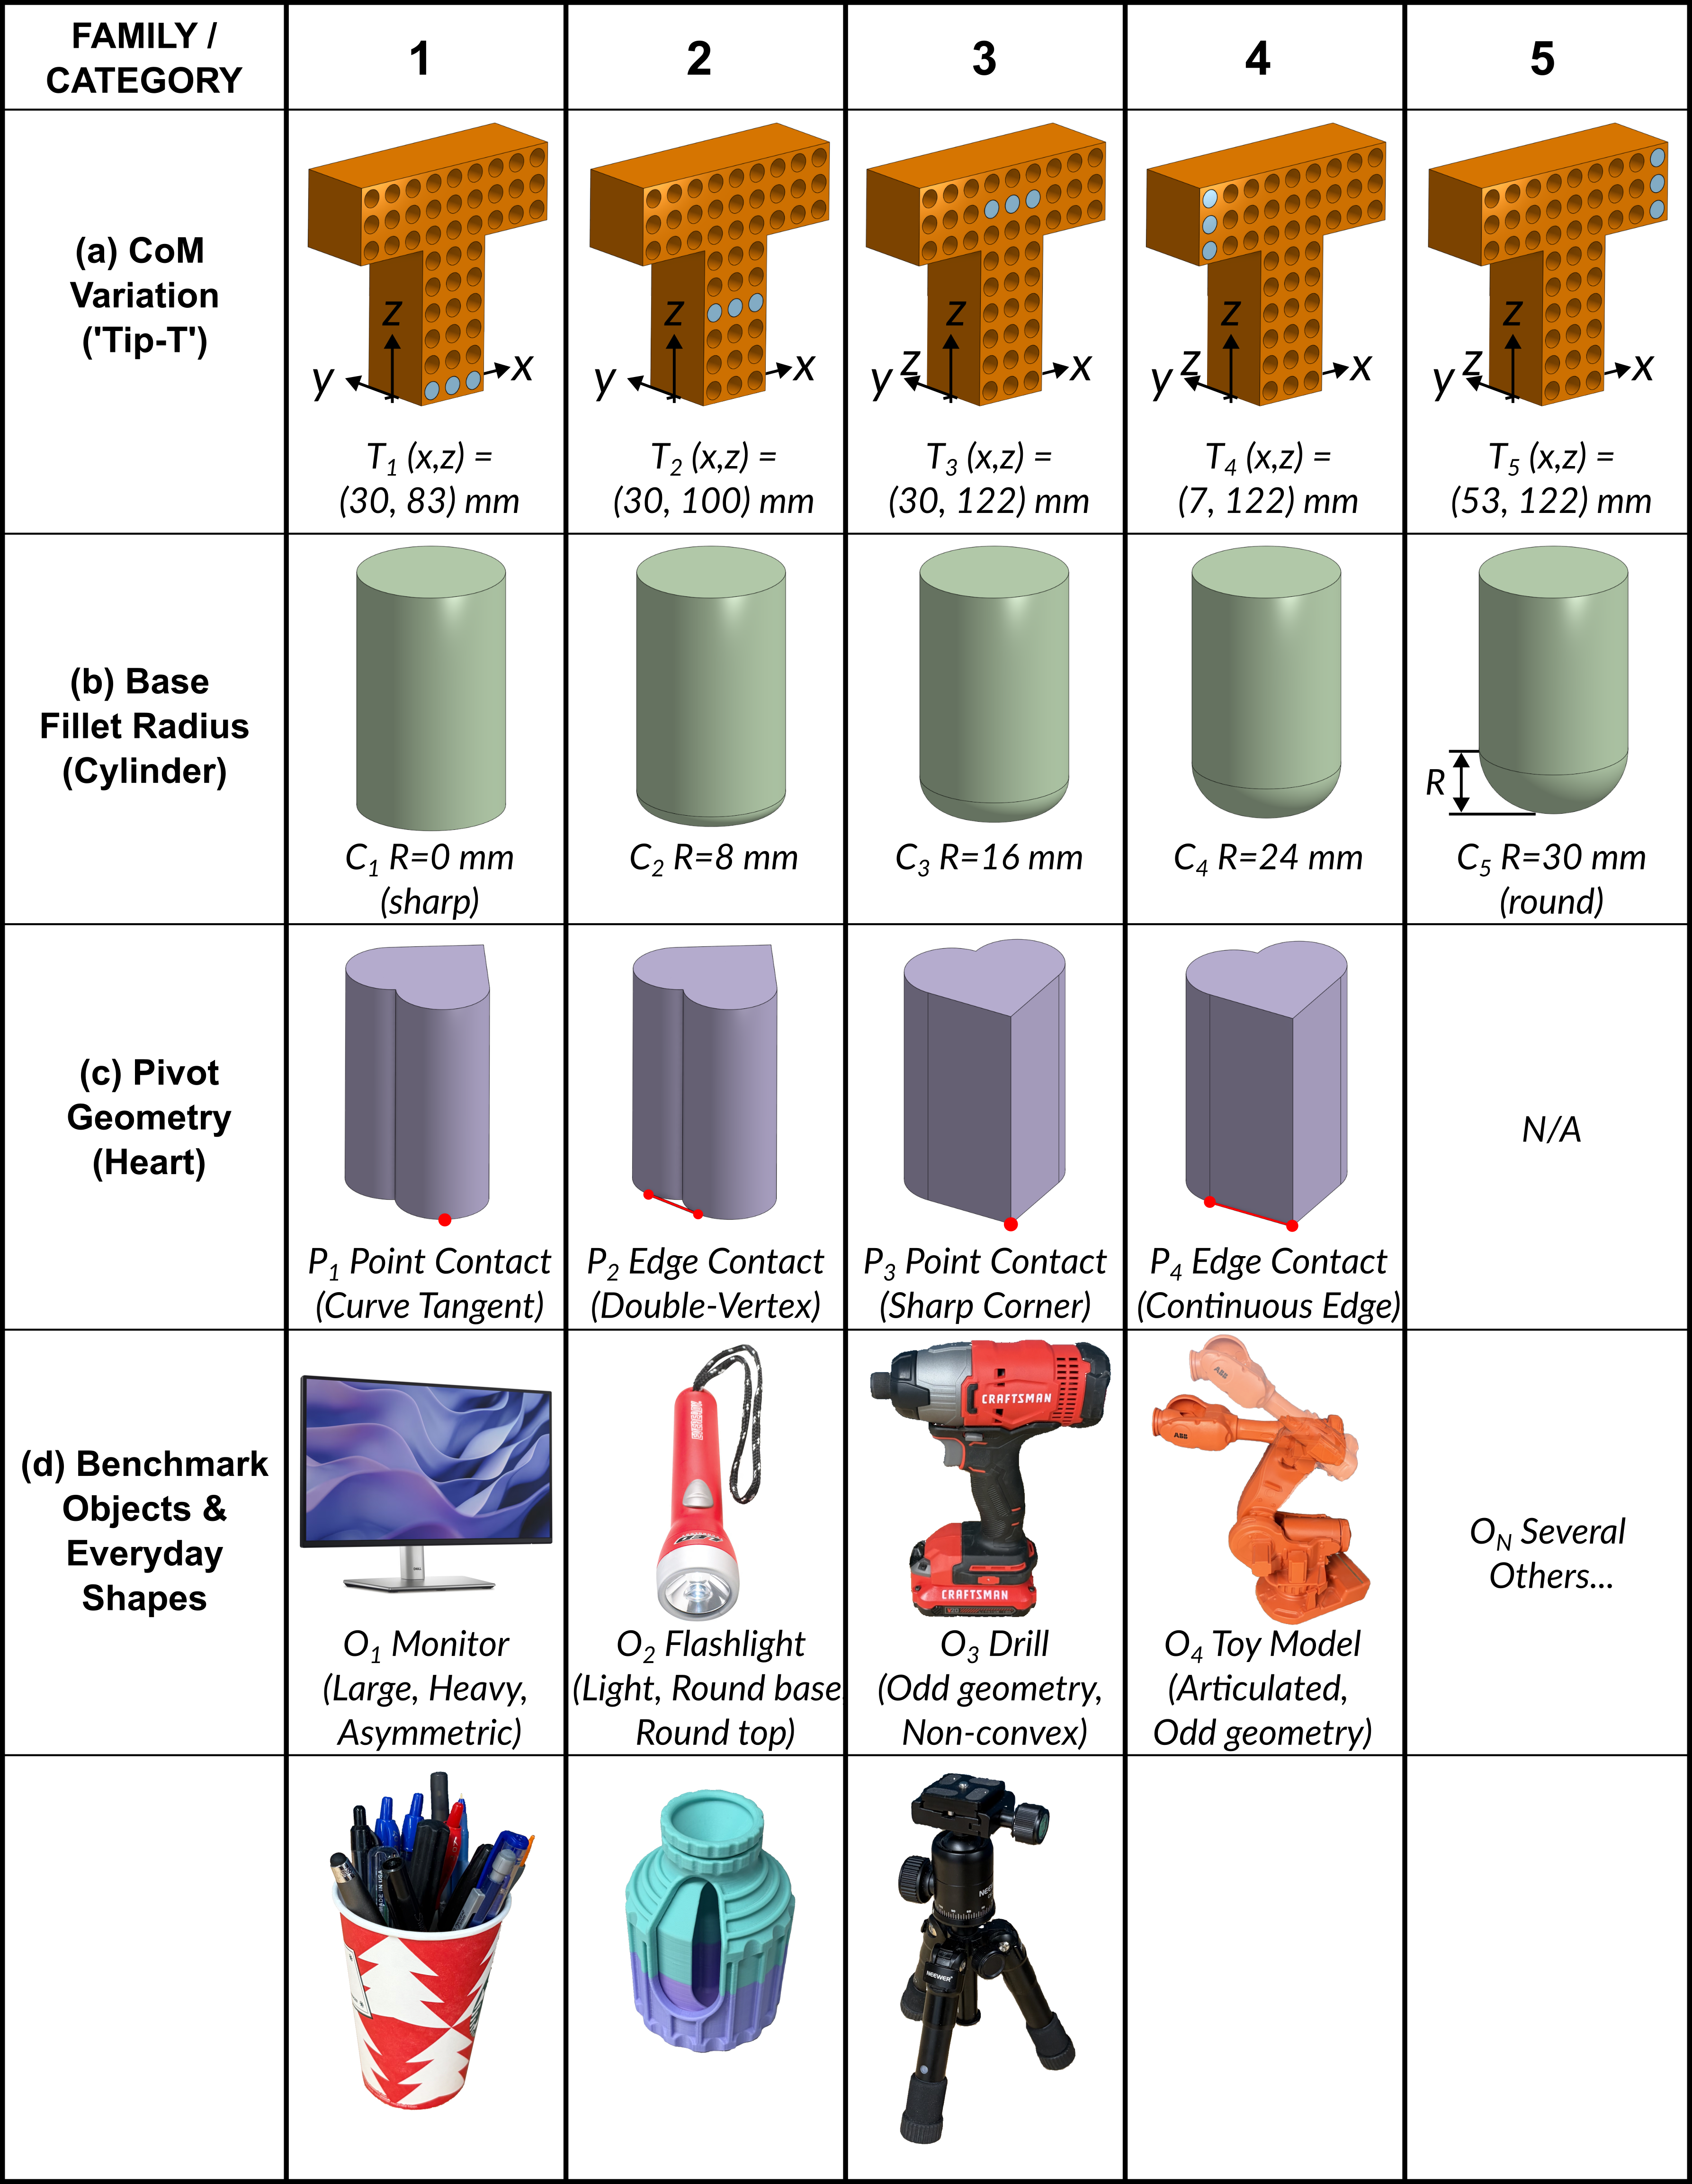
\includegraphics[width=0.95\linewidth]{figures/lineup.png}
  \caption{Object set. (a) CoM variation (Tip-T): one exterior, five slug placements. (b) Base fillet radius (cylinder), sharp to fully round. (c) Pivot geometry (heart): point and edge contacts. (d) Benchmark and everyday objects. \sh{Update the Tip-T labels to the current GT: $T_1$ (30, 82.47), $T_2$ (30, 99.4), $T_3$ (30, 122.0), $T_4$ (7.4, 122.0), $T_5$ (52.6, 122.0)\,mm; the figure still shows the old CAD heights 84.67/101.6/124.2. Add the friction series row.}}
  \label{fig:lineup}
\end{figure}

\subsection{Protocol}
For every configuration the robot runs the full pipeline autonomously: perceive, planar push, mode selection, tip with the recovery cascade, and re-perceive. Every episode logs the selected mode, the available candidates, the geometry terms ($d$, $h$, $a$, $L$), the friction priors, CoST and $p_{\min}$, which step decided, the execution outcome, and the fit quality. The evaluated object set, thresholds, calibration, and estimator version are frozen after a development pilot and before evaluation; all failures are reported and attributed to perception and contact selection, execution, estimation, or the downstream task where evidence permits. \sh{N trials per object/configuration: proposal 5 per estimation configuration, 10 per shove policy on the key pair. Decision: autonomous mode selection for every sweep configuration, or only for the everyday objects? Proposal: every configuration, since it is logged anyway.}

\noindent \textbf{Condition studies.} One study per swept axis: CoM offset (Tip-T), base rounding (cylinder fillets), pivot geometry (heart), base friction (bottom material), and contact placement (selected vs.\ centroid, random, and deliberately poor placements). Fingertip friction is held fixed with a single rubber tip; the monitor's fingertip slip is the reported limit.

\noindent \textbf{Safety study.} Retry and failure rates for the margin against the earlier reactive scheme, including at least one tip driven cleanly past the balance point; and a small sweep of more and less aggressive stopping points (press-and-pull arc limit; forward-tip $\eta_{\mathrm{safety}}$), similar to \iros{}, to build the safety--accuracy curve.

\subsection{Preliminary results: forward tipping on the Tip-T} \label{sec:prelim}
\sh{Everything in this subsection is pre-freeze, one trial per configuration (plus three repeats of tipT\_c), and will be replaced by the campaign. Kept here because it already supports several claims and exposes a systematic bias we must report.}

\noindent \textbf{Vision labels the outcome.} On all five Tip-T configurations the side camera correctly told what the object did (Table~\ref{tab:vision_labels}), including tipT\_e, where the CoM sat so close to the forward pivot that the contact force peaked at about 0.10\,N, below the force sensor's then-contact threshold. Slide distances from three independent sources agree: vision / finger travel / point clouds gave 34.9 / 35.3 / 37.5\,mm (a), 5.7 / 7.0 / 7.3\,mm (b), and 0.1 / 0.0 / $-1.0$\,mm (c).

\begin{table}[t]
  \centering
  \caption{What the object did, labeled by the side camera, against the proprioceptive pipeline (tipT a--e, 2026-10-13).}
  \label{tab:vision_labels}
  \small
  \begin{tabular}{l p{0.36\linewidth} p{0.34\linewidth}}
    \toprule
    & \textbf{Vision} & \textbf{Proprioceptive pipeline} \\
    \midrule
    a & Slid 34.7\,mm, then tipped to $13.2^\circ$ & Finger travel before onset 35.3\,mm, then tipped \\
    b & Slid 5.8\,mm, then tipped to $13.7^\circ$ & Finger travel 7.0\,mm, then tipped \\
    c & Tipped to $10.3^\circ$, no slide & Tipped \\
    d & Pure slide of 63.7\,mm, tilt $\le 1.0^\circ$ & Never rocked; skipped \\
    e & Tipped to $13.9^\circ$, no slide & Contact not found (0.10\,N peak) \\
    \bottomrule
  \end{tabular}
\end{table}

\noindent \textbf{CoST predicted the slides.} With the measured $\mu_t \approx 0.15$--0.17 from planar pushes, \eqref{eq:cost} gave 0.97--1.02 for a--c (marginal; a and b slid before tipping) and 0.56 for d, a predicted slide. tipT\_d's CoM is far from the forward pivot and therefore close to press-and-pull's pivot, so press-and-pull should succeed; tipT\_e's $d$ is below the observability gate. Both failures were predictable before any motion. \sh{Rerun d and e with the current controller: expect slide $\rightarrow$ press-and-pull, and too easy $\rightarrow$ press-and-pull.}

\begin{figure*}[t]
  \centering
  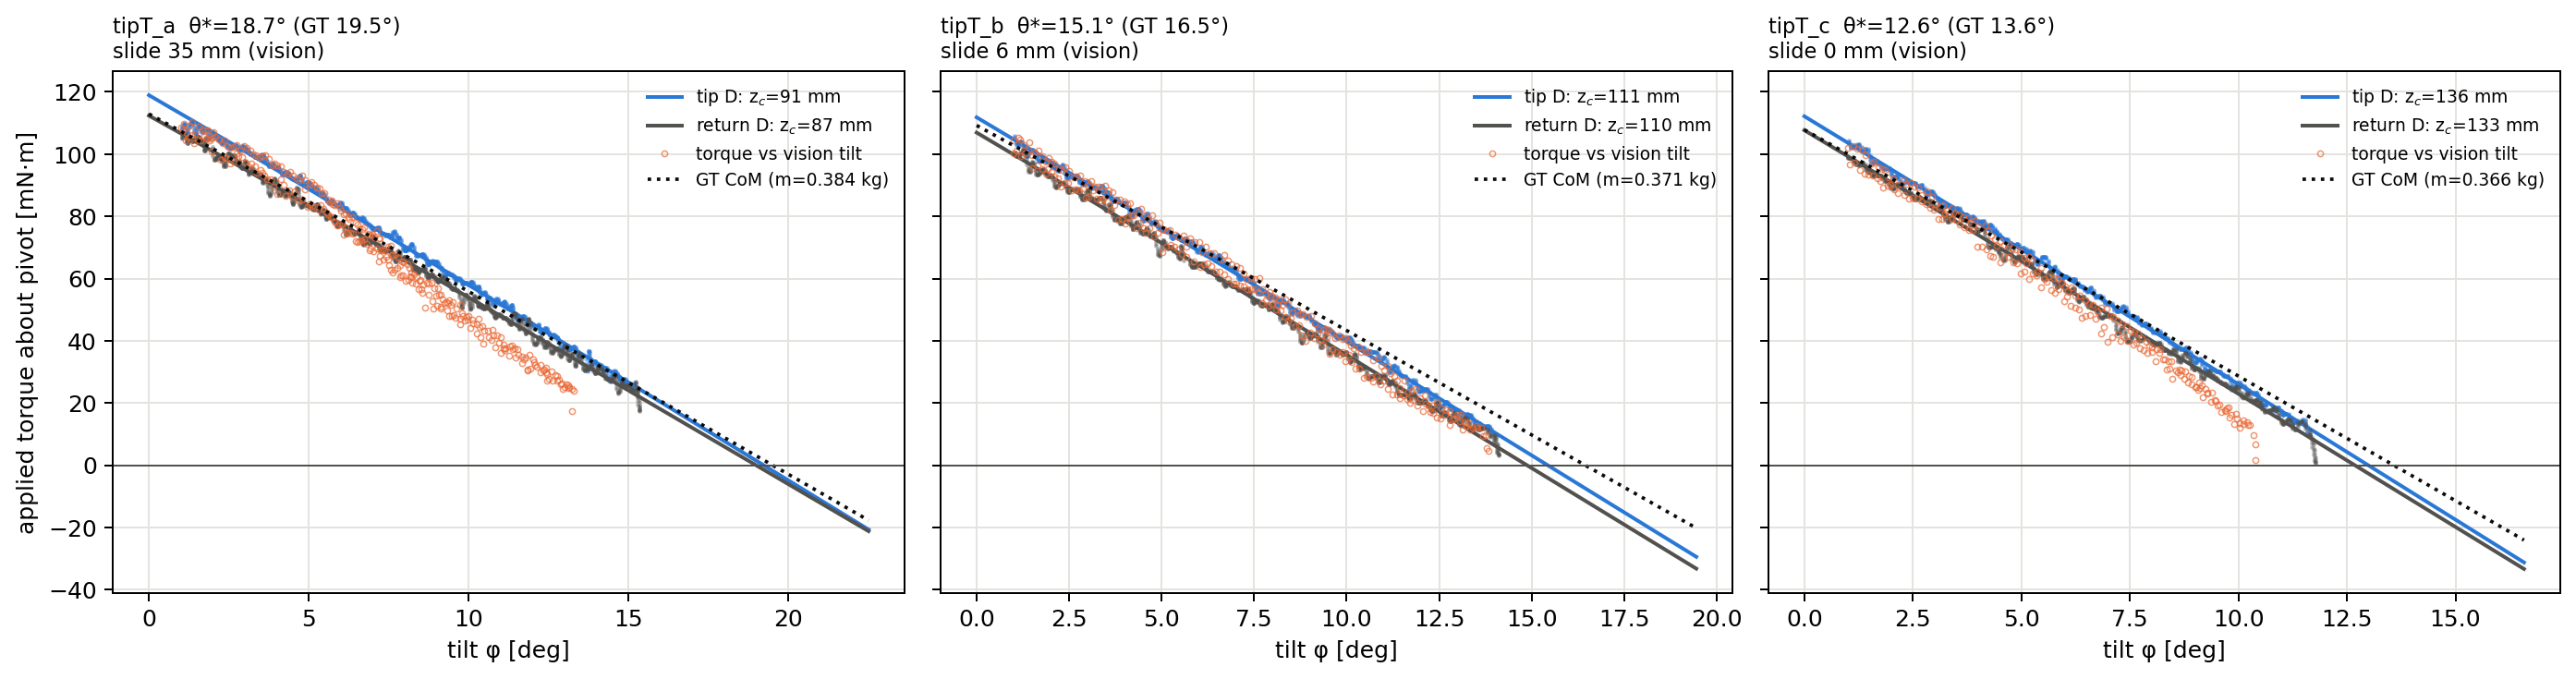
\includegraphics[width=0.95\textwidth]{figures/runtime_logs/fwd_tip_fits.png}
  \caption{Forward tipping, torque about the pivot against tilt for tipT a--c. Method D fits on the push (blue) and return (gray) branches, torque against vision tilt (orange), and the ground-truth curve (dotted). tipT\_a slid 35\,mm before tipping and still produced a usable fit. \sh{Source: runtime\_logs/tipT\_full\_suite/estimation\_fwd\_tip/fwd\_tip\_fits.png. Regenerate with the frozen estimator and current GT (the legend still shows the old GT masses).}}
  \label{fig:fwd_tip_fits}
\end{figure*}

\noindent \textbf{Proprioception beats vision for metric tilt.} Vision under-read tilt by 3--20\%. Because method D absorbs offsets but not scale, vision-only $z_c$ came out 14--30\% off, against 5--9\% for proprioception (against the GT of the time). The first-order theory holds: the ratio of vision-only to proprioceptive $\hat z_c$ was 1.235 / 1.041 / 1.119, against tilt scale ratios of 1.201 / 1.033 / 1.097 (Fig.~\ref{fig:fwd_tip_fits}).

\noindent \textbf{What is identifiable is accurate.} With the GT mass, the mass-weighted moment $m r$ was within 0.5 / 0.0 / 2.1\% for a / b / c, while $m$ alone was 5--9\% low. The effective in-board distance implied by the mass (28.6 / 27.7 / 27.3\,mm) matched the one implied by $z_c$ (28.6 / 27.5 / 27.7\,mm), against a geometric 30\,mm. Exactly as \eqref{eq:lambda_invariance} predicts, the estimator recovered the identifiable quantities, and the $m$ and $z_c$ errors trace to the conditioning input. \sh{These numbers used the old GT (403\,g; $z_c$ 84.7/101.6/124.2\,mm). Recompute with the current GT (404\,g; 82.47/99.4/122.0\,mm).}

\begin{table}[t]
  \centering
  \caption{Repeatability and the mass deficit on tipT\_c (GT 404\,g, $d = 30$\,mm, $z_c = 122$\,mm). Method D as currently implemented.}
  \label{tab:bias}
  \small
  \begin{tabular}{l r r r r}
    \toprule
    \textbf{Run} & $\hat m_D$ (g) & \textbf{Error} & $\hat m_B$ (g) & $\hat z_{c,D}$ (mm) \\
    \midrule
    c (original) & 366.4 & $-9.3\%$ & 373.5 & 134.3 \\
    c1 & 376.1 & $-6.9\%$ & 388.3 & 139.9 \\
    c2 & 375.7 & $-7.0\%$ & 380.8 & 137.5 \\
    c3 & 380.2 & $-5.9\%$ & 394.1 & 131.5 \\
    \bottomrule
  \end{tabular}
\end{table}

\begin{figure}[t]
  \centering
  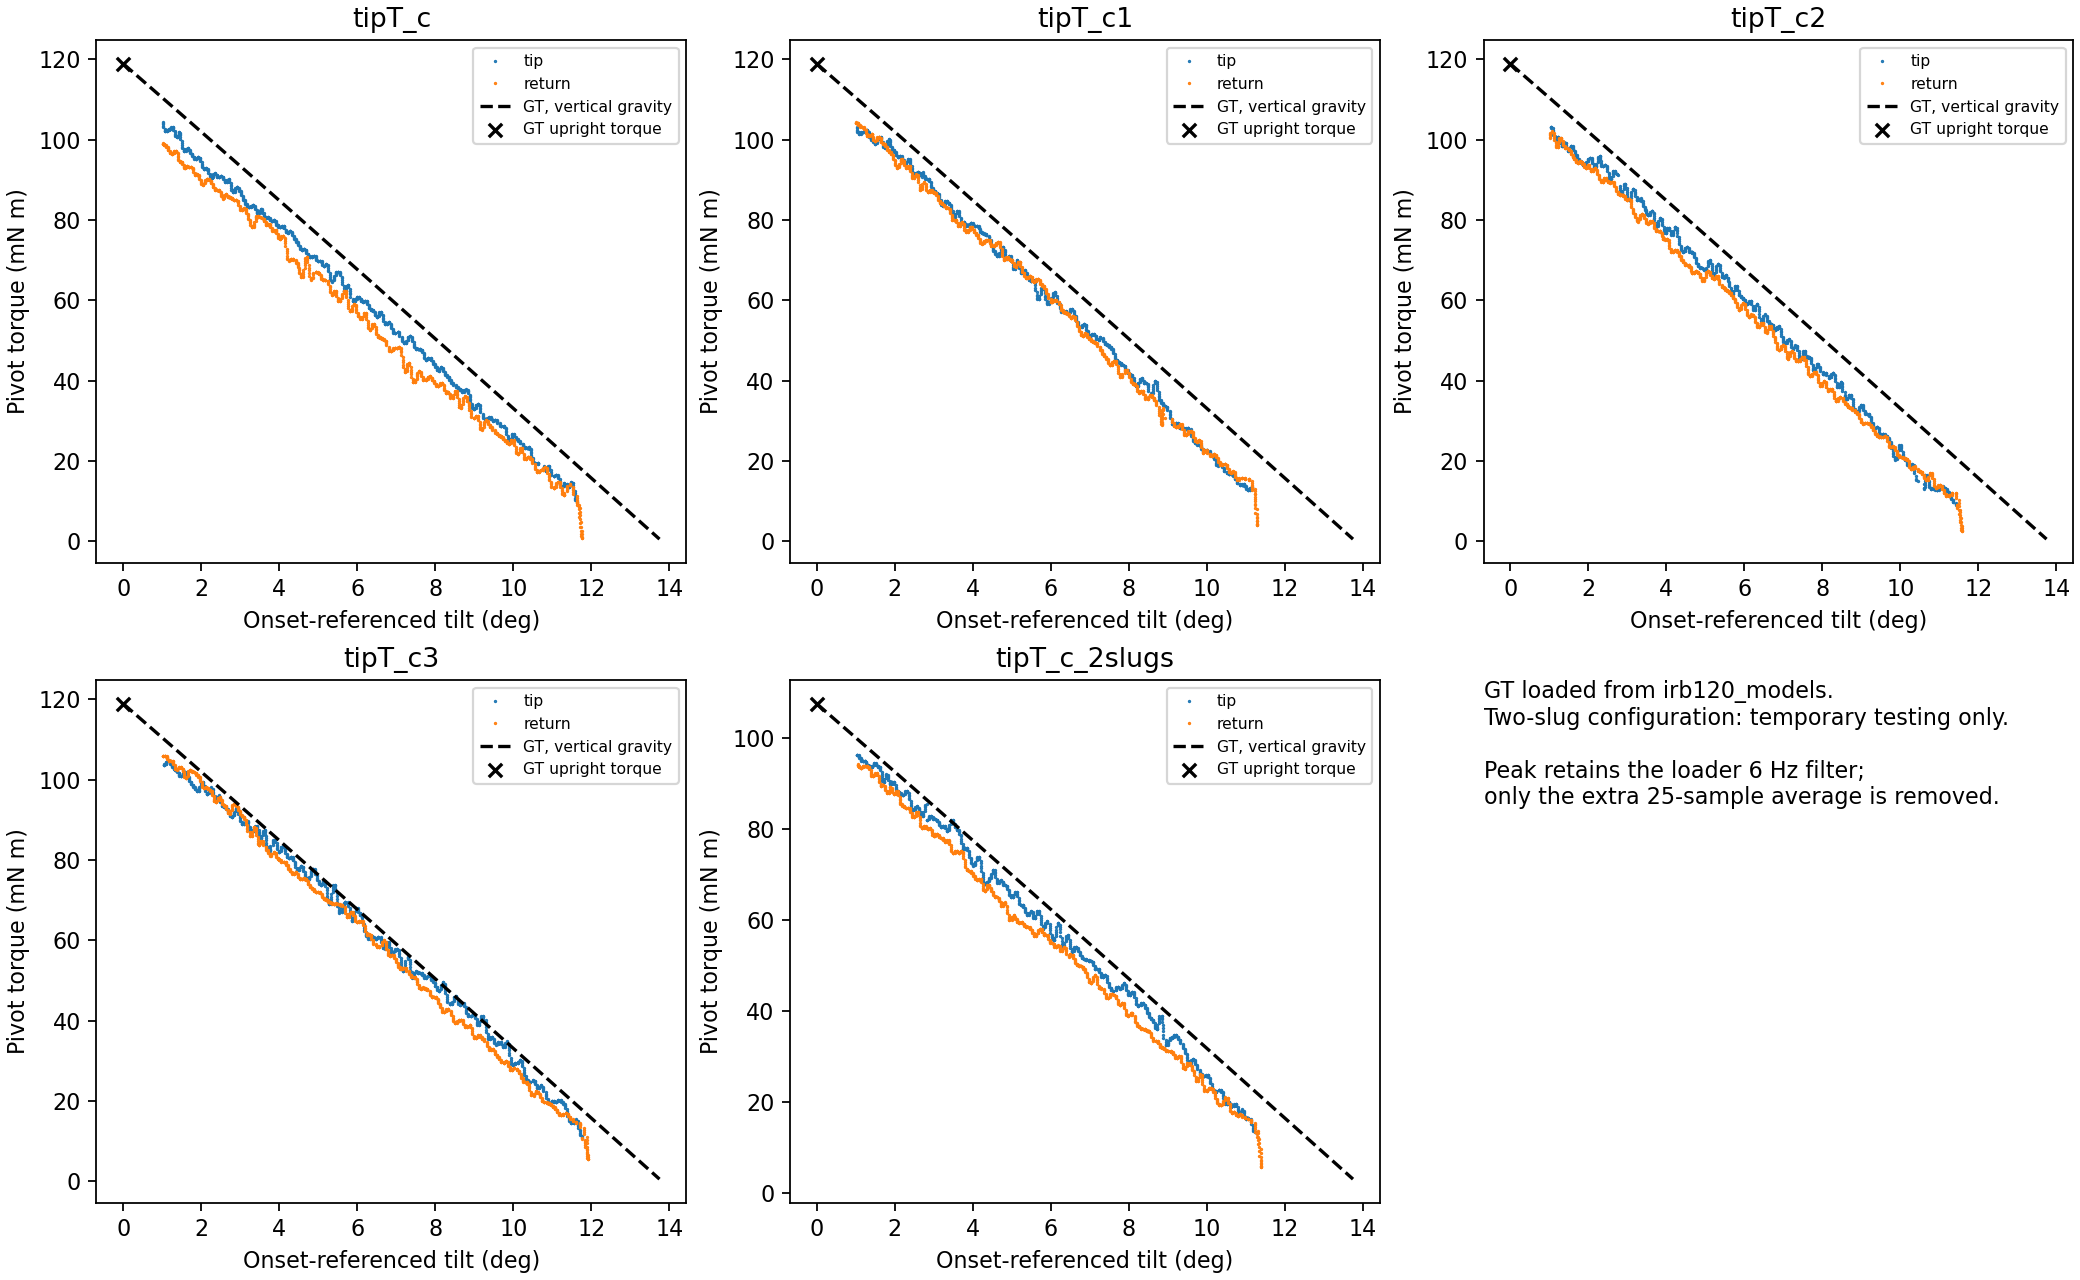
\includegraphics[width=0.95\linewidth]{figures/runtime_logs/torque_curves.png}
  \caption{Measured pivot torque against onset-referenced tilt for the tipT\_c repeats, against the ground-truth curve under vertical gravity. The deficit is systematic across repeats. \sh{Source: runtime\_logs/tipT\_bias\_audit/torque\_curves.png. Drop the temporary two-slug panel for the paper.}}
  \label{fig:torque_curves}
\end{figure}

\noindent \textbf{A systematic mass deficit, partly explained.} The three repeats average 377.3\,g with a sample standard deviation of 2.5\,g, so the 26.7\,g deficit is systematic, not noise (Table~\ref{tab:bias}, Fig.~\ref{fig:torque_curves}). Two contributions are confirmed. First, the estimator's extra moving average on the onset torque: removing it raises the masses to 382.4 / 379.6 / 384.5\,g. Second, a late zero: the side camera shows c1 already tilted $0.515^\circ$ at the selected torque peak, which alone accounts for about 4.35\,mN\,m; using that angle gives 396.9\,g. c3 shows no such tilt and retains a deficit. An in-plane tilt of the calibrated gravity vector ($0.33^\circ$) would account for about 2.8\,mN\,m but has not been independently verified. Small reference-pivot errors are excluded as the main cause: a 1\,mm vertical shift changes the residual by only 0.01--0.02\,mN\,m once the tilt is recomputed, whereas a \emph{physical} support edge displaced inboard by 1\,mm costs about 4\,mN\,m. The raw sensor stream, re-baselined independently of the tare, shows the same shortfall. We report the remainder as a bounded error rather than fit a correction to ground truth. \sh{Before the campaign: known-weight F/T gain check; decide whether to anchor onset on observed lift (vision) instead of the torque peak.}

\begin{figure}[t]
  \centering
  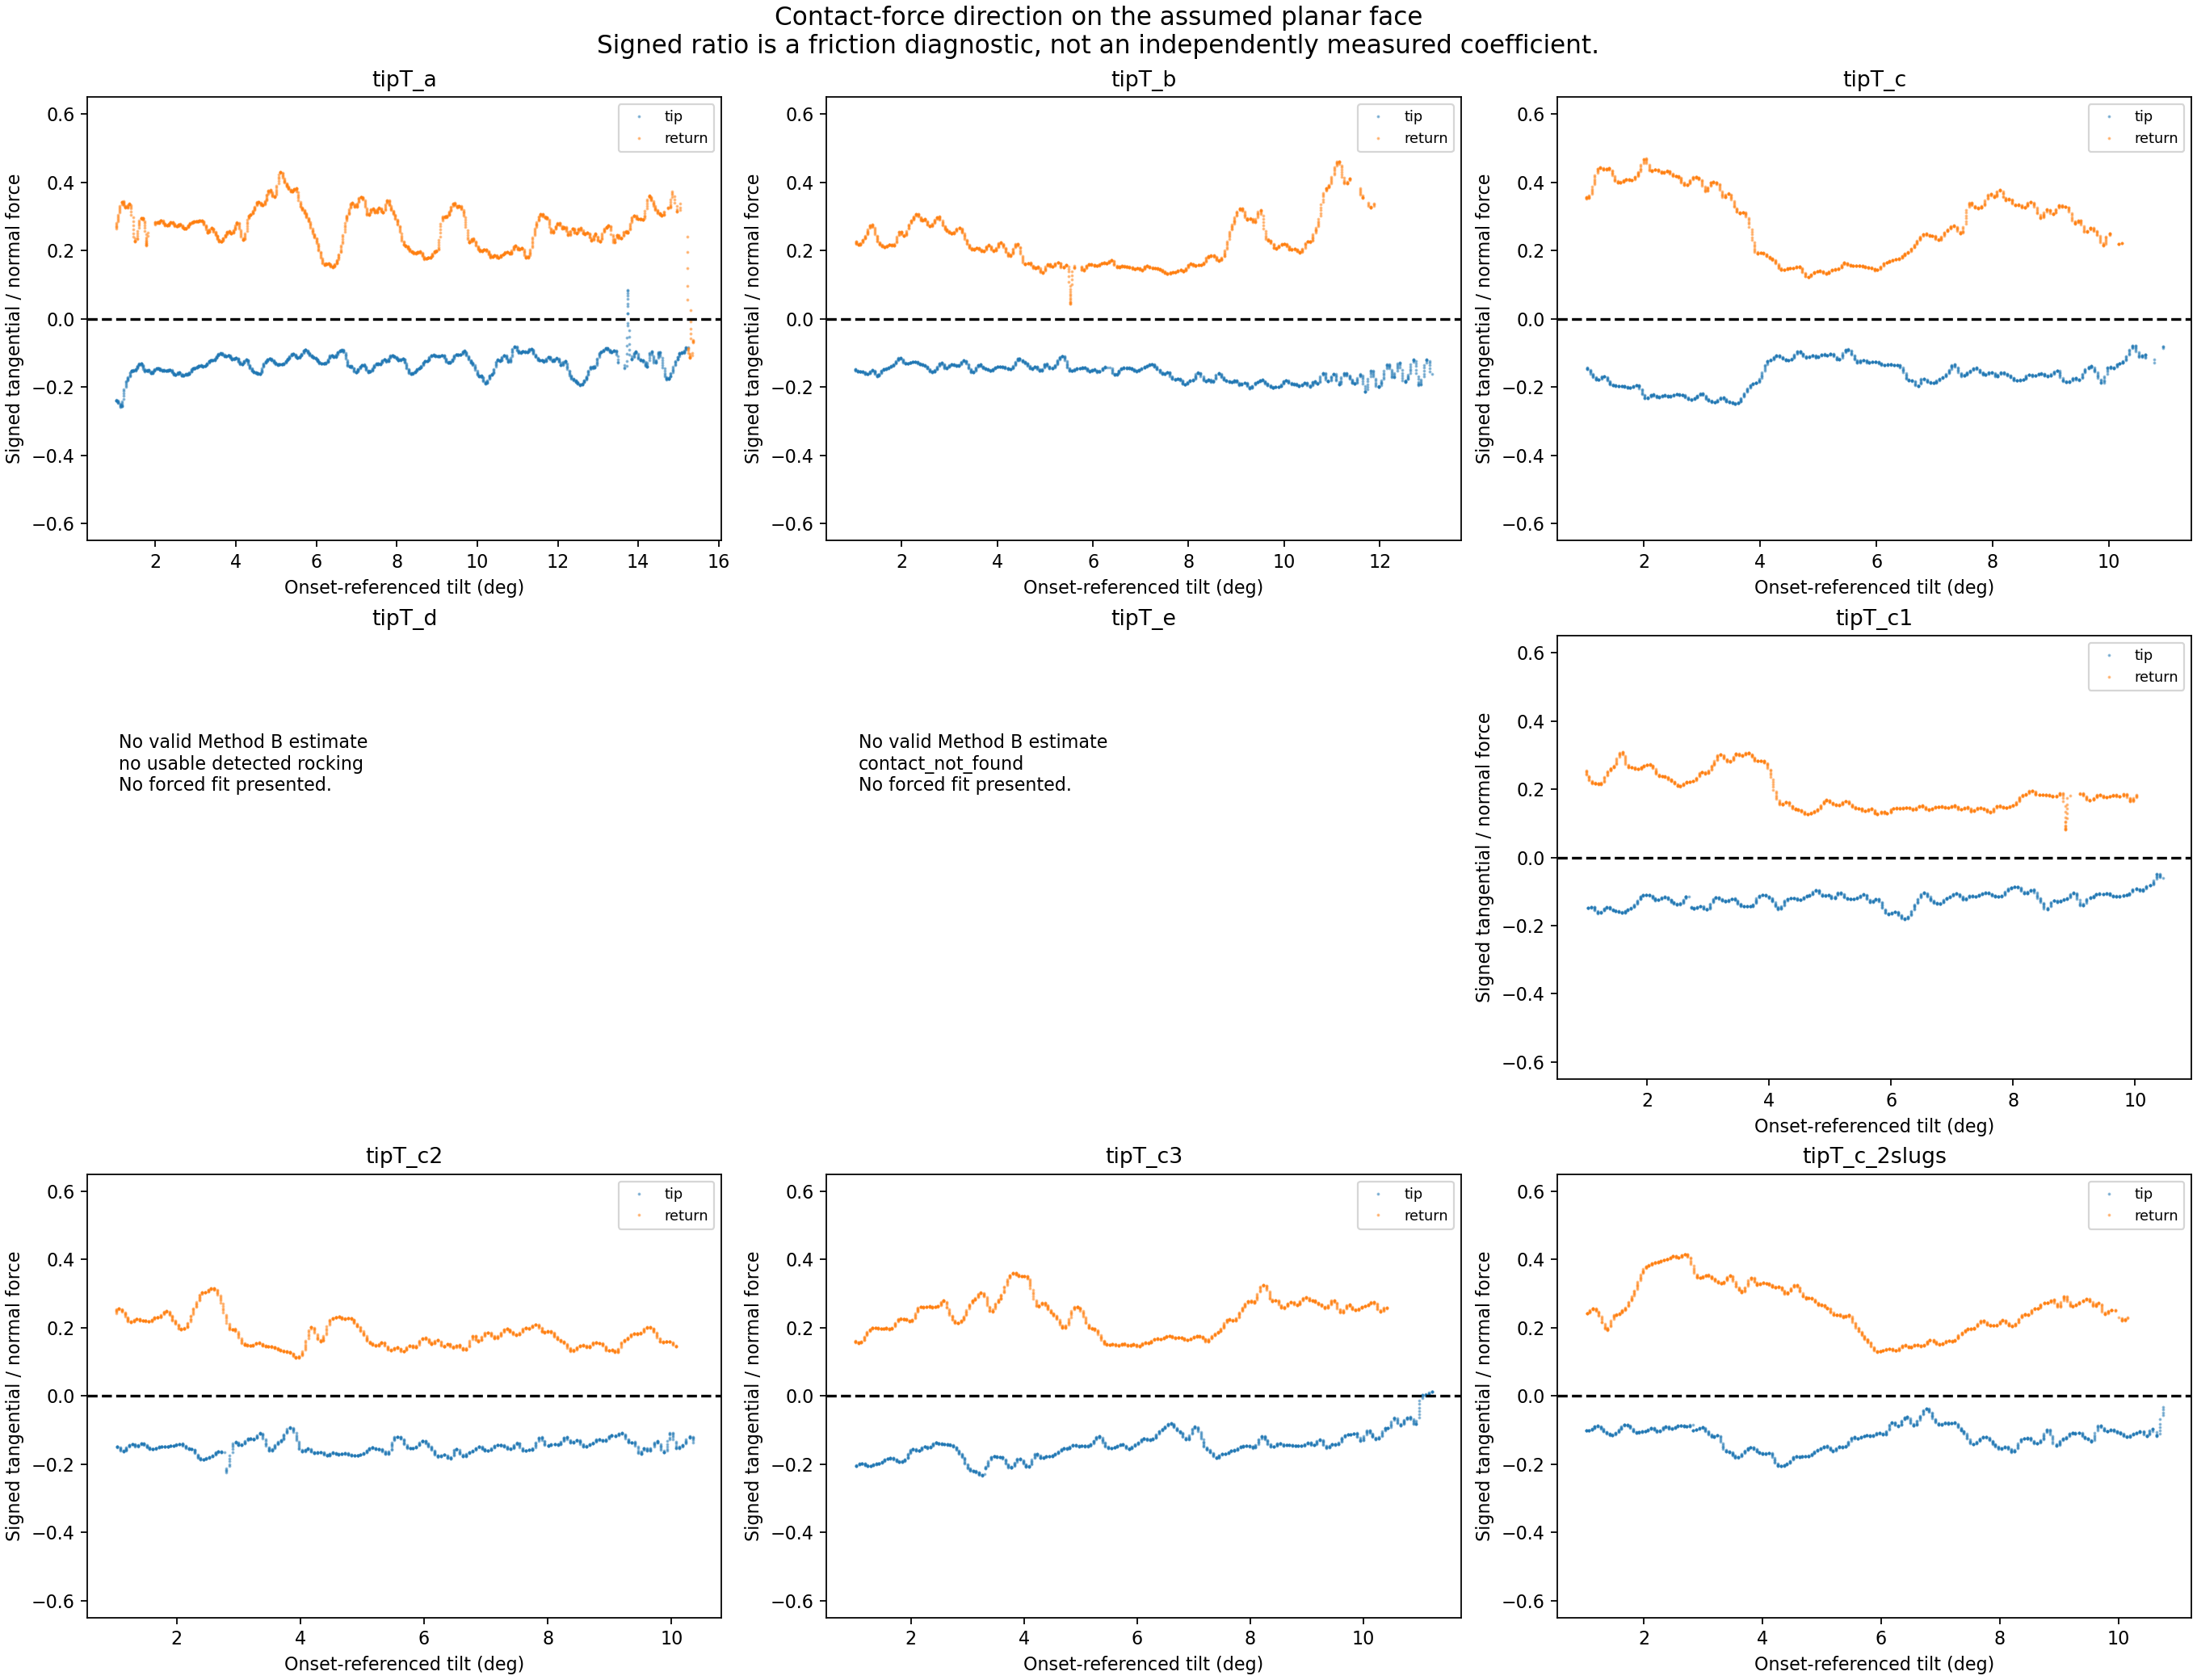
\includegraphics[width=0.95\linewidth]{figures/runtime_logs/contact_friction_diagnostic.png}
  \caption{Contact-force direction on the assumed planar face: signed tangential over normal force at the fingertip, push (blue) and return (orange). The ratio stays within about $\pm0.4$, inside the fingertip's friction cone, supporting the sliding-ball contact model used for proprioceptive tilt. This is a friction diagnostic, not an independently measured coefficient. \sh{Source: runtime\_logs/tipT\_bias\_audit/contact\_friction\_diagnostic.png. Optional; supplementary material?}}
  \label{fig:contact_friction}
\end{figure}

\subsection{Multi-modal accuracy}
Table~\ref{tab:results} reports estimated $(m, z_c, \mu_t)$ against ground truth across the full set. We expect the heavier objects to yield the cleanest estimates, as a larger gravitational torque produces a higher signal-to-noise wrench trajectory during tipping, and the light, sliding, poor-top regime to be hardest, consistent with the conditioning analysis of Section~\ref{sec:conditioning}. \sh{Fill from the campaign.}

\begin{table}[t]
  \centering
  \caption{Estimation results on physical objects. \sh{Fill from data; add $m r$, mode chosen, and attempts.}}
  \label{tab:results}
  \small
  \begin{tabular}{l ccc ccc}
    \toprule
    & \multicolumn{3}{c}{\textbf{Ground truth}} & \multicolumn{3}{c}{\textbf{Rel.\ error (\%)}} \\
    \cmidrule(lr){2-4}\cmidrule(lr){5-7}
    \textbf{Object} & $m$ & $z_c$ & $\mu_t$ & $|\Delta m|$ & $|\Delta z_c|$ & $|\Delta\mu_t|$ \\
    \midrule
    \sh{fill} & [\,] & [\,] & [\,] & [\,] & [\,] & [\,] \\
    $\vdots$ &      &      &      &      &      &      \\
    \bottomrule
  \end{tabular}
\end{table}

\subsection{Where the method stops working}
Each sweep isolates a single claim and yields a degradation curve and a stated breakdown point, so the conclusions can give the envelope numerically. CoM offset: $d \to 0$ (tipT\_e) is the observability breakdown and large $d$ (tipT\_d) is the slide breakdown, a two-sided envelope. Base fillet radius: we sweep from sharp to fully round and report estimation quality against radius, mapping where the fixed-pivot assumption degrades rather than claiming arbitrary curved bottoms are solved; the roundness threshold of Step~1 is set here. Pivot geometry: point and edge contacts of the heart series probe the assumption that the pivot is a well-defined line. Base friction: same geometry and mass, different bottom materials, to set the sliding-limit margin $\epsilon$ of Step~2 and check CoST per material.

\begin{figure}[t]
  \centering
  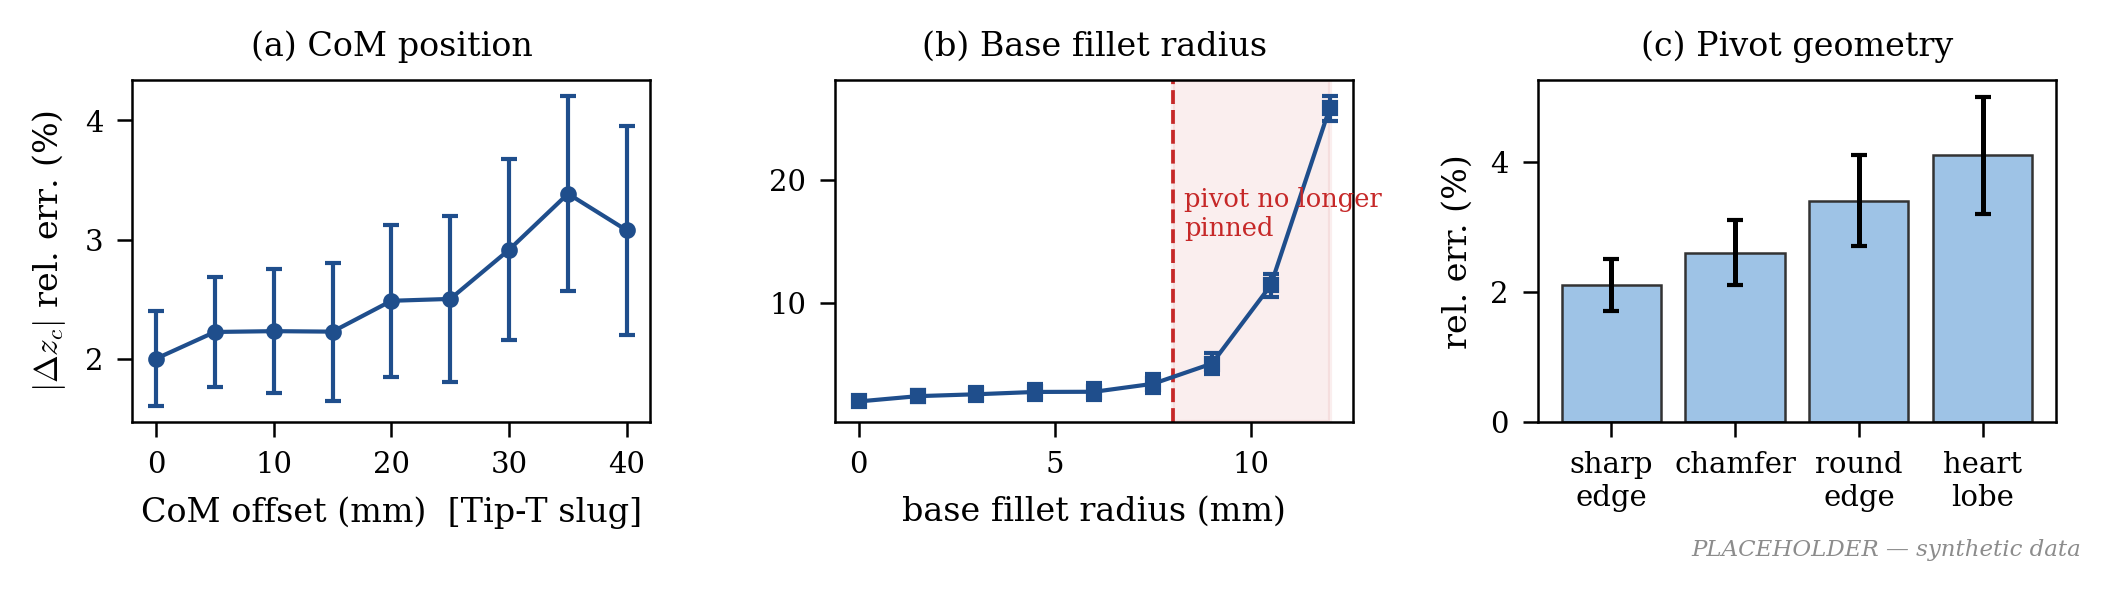
\includegraphics[width=0.95\linewidth]{figures/fig5_sweeps.png}
  \caption{Parametric sweeps. Estimation error versus (a) CoM offset, (b) base fillet radius, and (c) pivot geometry. \sh{PLACEHOLDER with synthetic data: replace with campaign data, and add (d) base friction.}}
  \label{fig:sweeps}
\end{figure}

\subsection{Mode choice and contact placement}
\sh{For every object: which mode the heuristic picked, which step decided, and whether the choice held up (attempts used, cascade reasons). Contact ablation: selected vs.\ centroid, random, and deliberately poor placements, 3 placements $\times$ 2 objects $\times$ 3 trials. Show the hard case here, with its prediction stated before the result.}

\subsection{Safety framework validation}
\sh{Margin traces $\lambda_{\mathrm{slip}}(\theta)$ and $\lambda_{\mathrm{topple}}(\theta)$ for representative press-and-pull tips, including at least one driven cleanly through $\theta^{*}$ (the thesis-defining trace); retry and failure rates against the ISRR reactive scheme; safety--accuracy curve from the arc-limit sweep.}

\begin{figure}[t]
  \centering
  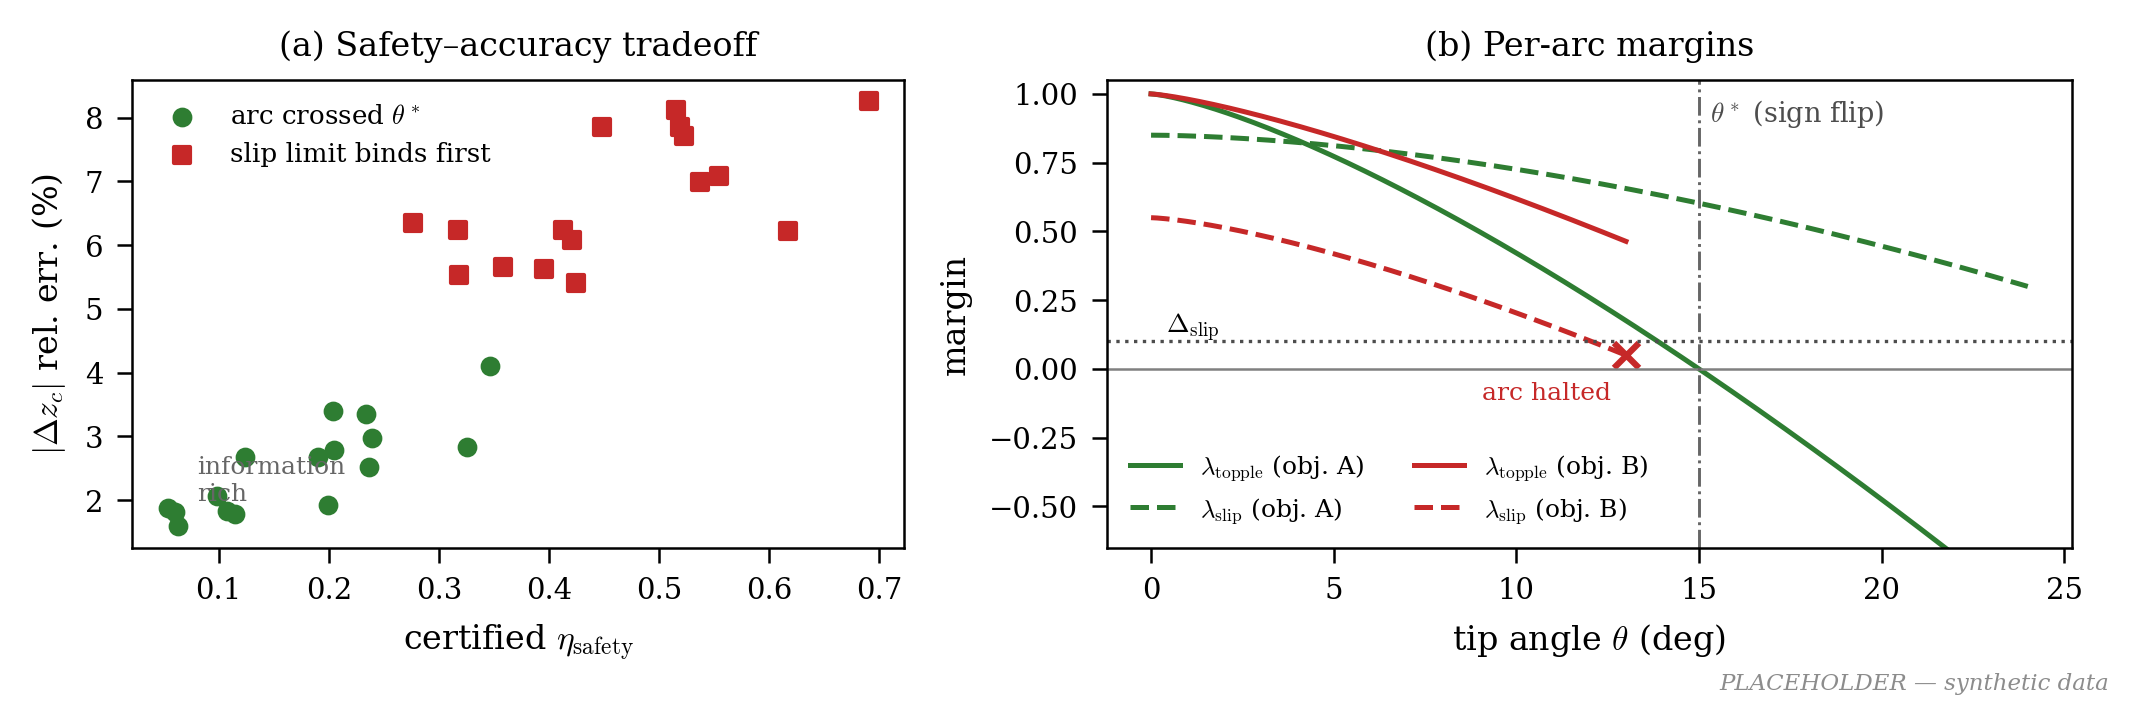
\includegraphics[width=0.95\linewidth]{figures/fig6_tradeoff.png}
  \caption{Safety--accuracy tradeoff. (left) Estimation error versus the certified margin. (right) Per-arc margins $\lambda_{\mathrm{topple}}(\theta)$ and $\lambda_{\mathrm{slip}}(\theta)$, illustrating objects whose slip budget admits crossing $\theta^{*}$ and objects where the slip limit binds first. \sh{PLACEHOLDER with synthetic data. Relabel the x-axis $\eta_{\mathrm{slip}}$ (not $\eta_{\mathrm{safety}}$) to match the renamed margin.}}
  \label{fig:tradeoff}
\end{figure}

\subsection{Complete-pipeline demonstration}
For one object we run planar $(x_c, y_c)$ estimation end to end, without a supplied planar CoM, so the full pipeline is exercised; the rest follow identically. This demonstrates completeness and is not a contribution of this work. \sh{Which object? With video.}

\subsection{Comparison}
\sh{Keep the qualitative capability table from OLDmain (method families: press-and-pull, multi-tip/GEEP, forward tipping, grasp-based excitation, planar pushing, tactile, vision/learned, VLM + interaction); add a column for mode selection and one for interactions required. Quantitative: forward-only vs.\ press-and-pull-only vs.\ selected mode on identical objects. A full Yu et al.\ reproduction is out of scope (it needs matched material-point measurements and three independent supports); compare interaction counts and cite their reported accuracy.}

%% ==============================================
\section{Validation: Parameter-Gated Dynamic Shoving} \label{sec:validation}
%% ==============================================

Accurate parameters are only useful if they change what the robot can safely do. We therefore close the loop with a downstream task whose success is gated by the estimated parameters: a dynamic shove that drives an object into a target planar region, upright, in a single push. The shove is the only dynamic motion in the paper; it also tests whether quasistatically recovered parameters transfer to a dynamic regime. \jx{The assumptions about the objects should be the same as the ones about the objects that we can estimate the physical properties.} \jx{Shoving has to occur within the workspace of the fixed-base manipulator, but the distance moved after shoving depends on the friction of the table and the object. Un-shovable objects like the monitor?}

\begin{figure}[t]
  \centering
  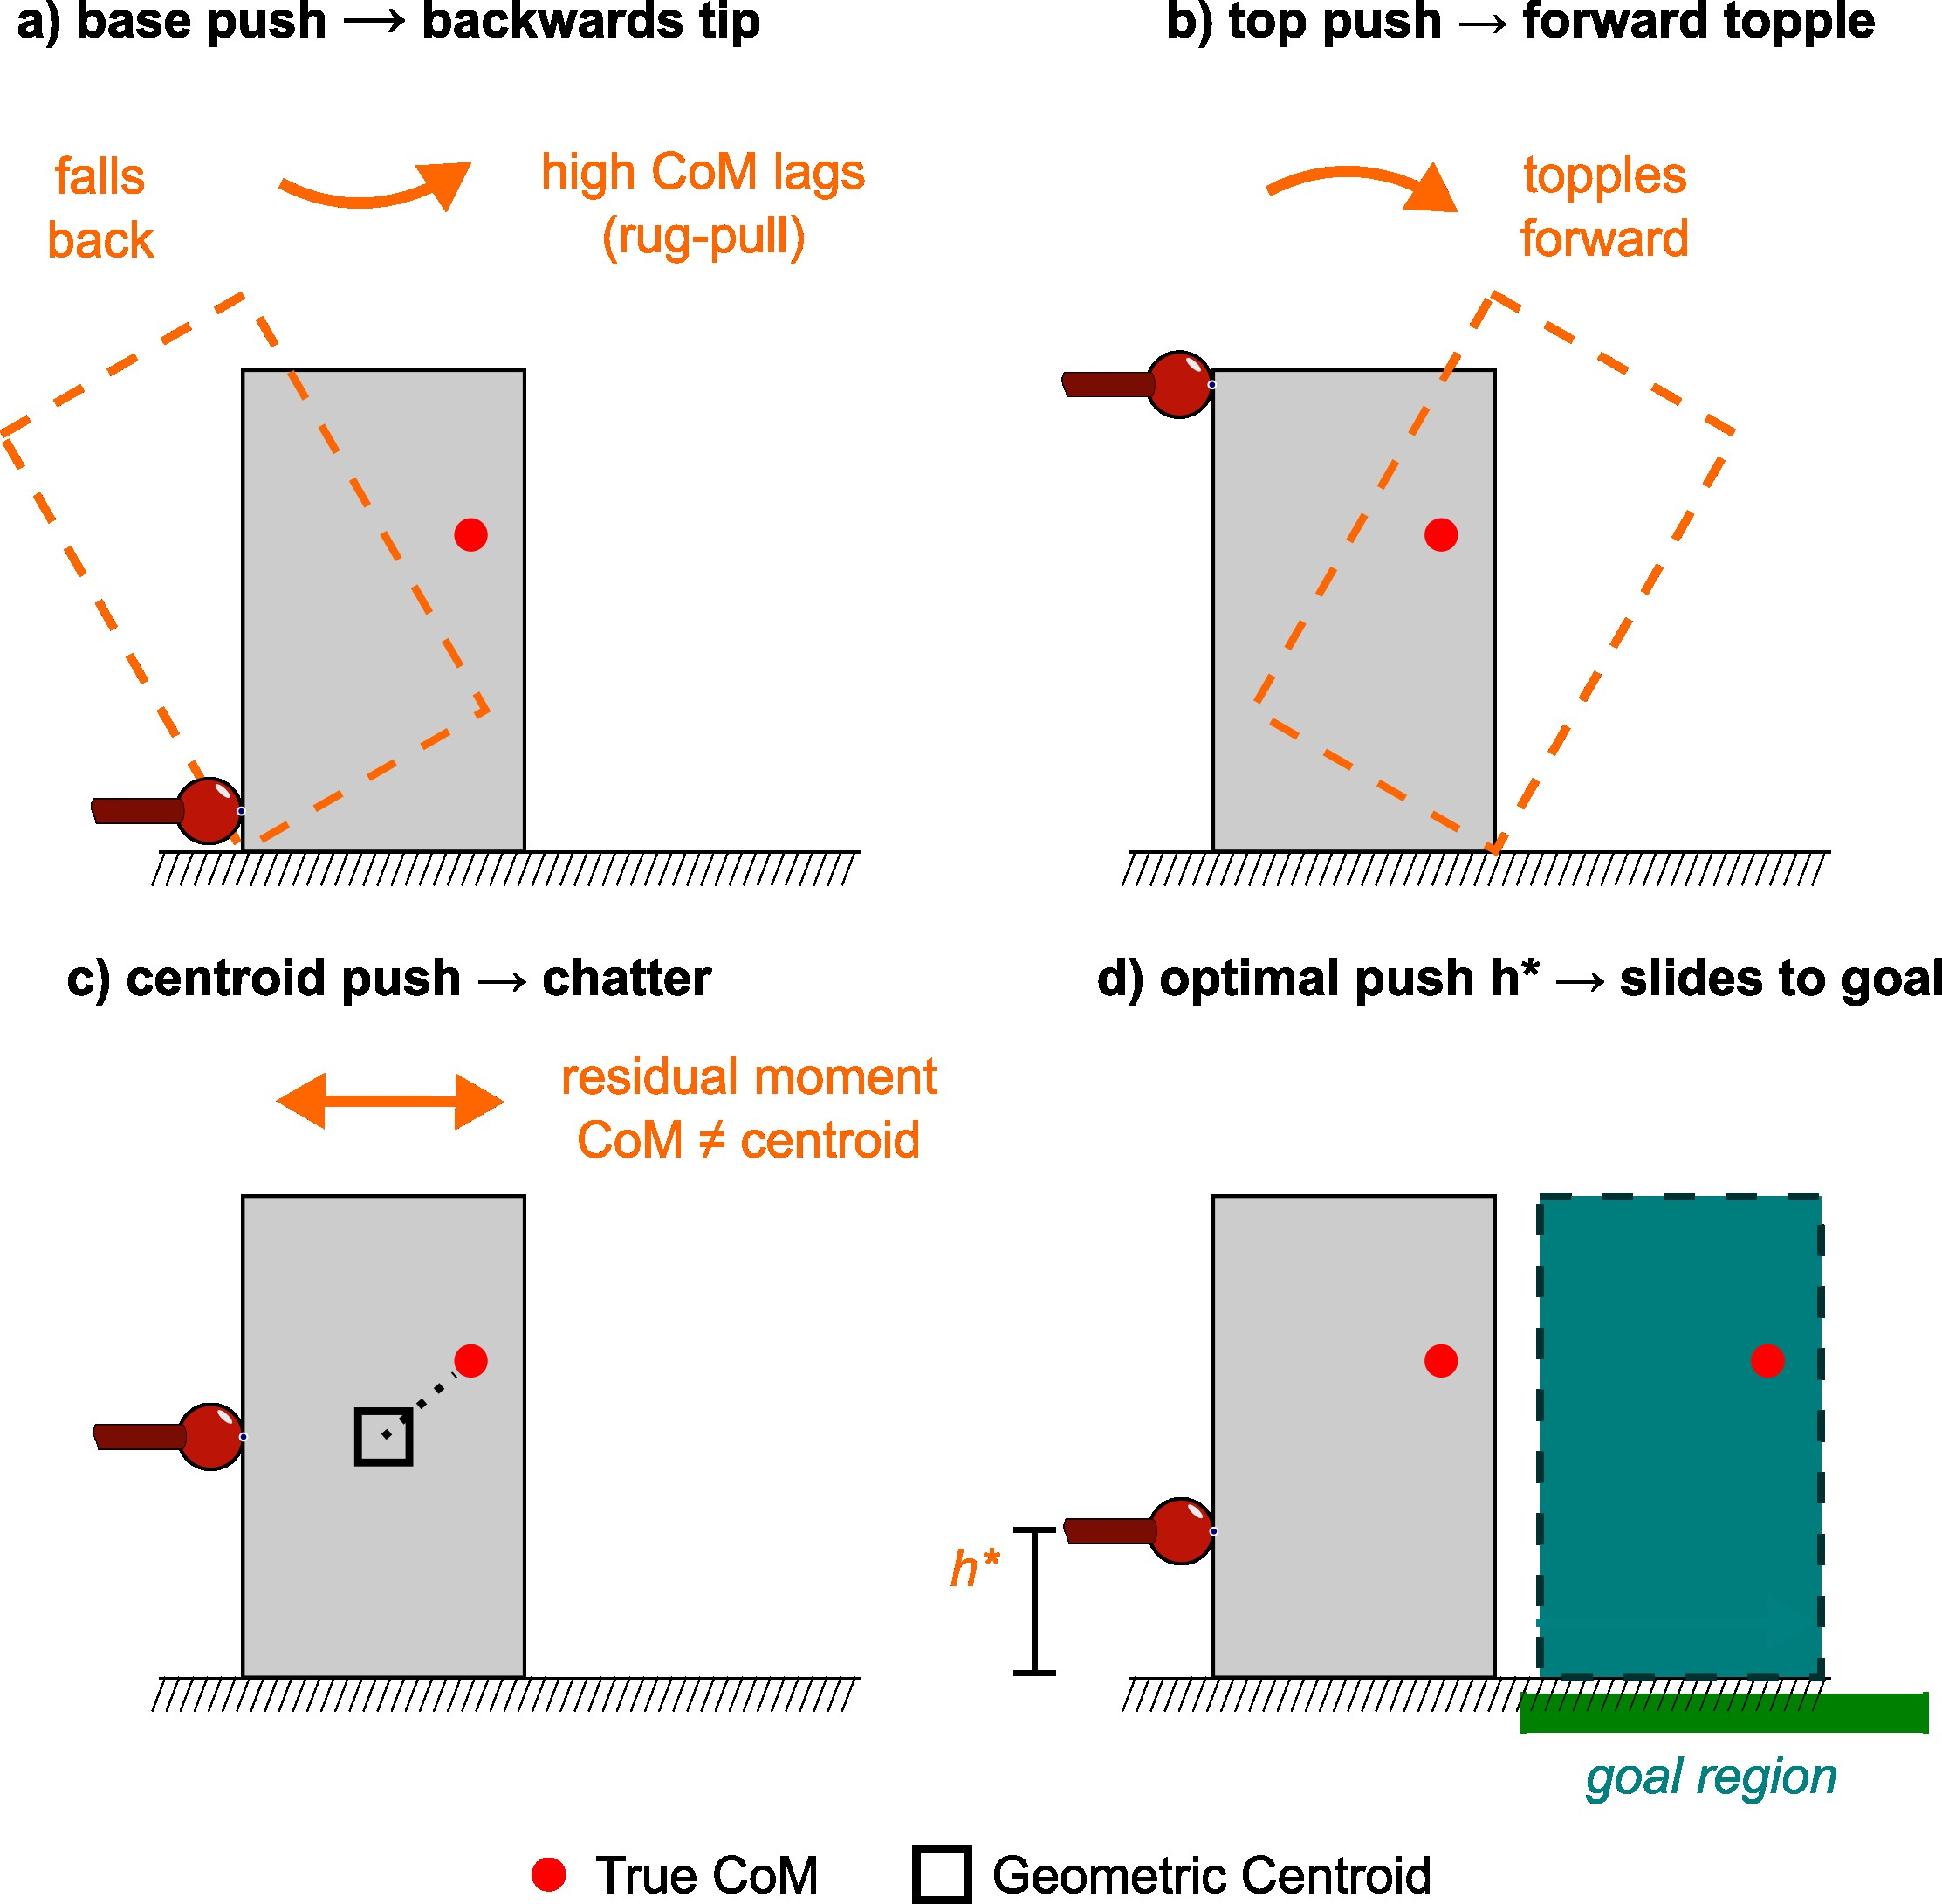
\includegraphics[width=0.98\linewidth]{figures/shove_validation.jpg}
  \\[4pt]
  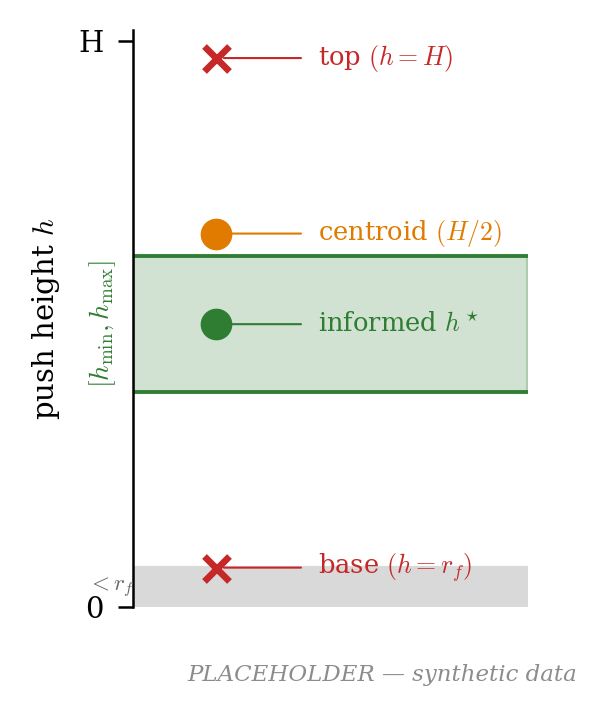
\includegraphics[width=0.6\linewidth]{figures/fig7_inset_window.png}
  \caption{Parameter-gated shove-to-region validation. Uninformed geometry-only push heuristics fail in distinct ways on a high-CoM, non-uniform object: a base push tips it backward (the high CoM lags), a top push topples it forward (base friction pins the bottom), and a centroid push chatters because the true CoM is offset from the geometric centroid. The informed push, inside the estimated no-tip window, slides the object into the target. (inset) The admissible push-height window. \sh{From the old draft and illustrative (the ISRR shove video was simulated); replace with hardware frames.}}
  \label{fig:shove}
\end{figure}

\noindent \textbf{No-tip condition and admissible push height.} We work in the vertical plane containing the push. Let the support base reduce to the segment $[-d_r, d_f]$, where $d_r$ and $d_f$ are the horizontal distances from the CoM's vertical projection to the trailing and leading bottom edges; non-uniform density appears precisely as an asymmetry $d_f \neq d_r$. The object slides under a horizontal shove of constant acceleration $a$ when
\begin{equation}
    F = m\,(a + \mu_t g).
    \label{eq:shove_force}
\end{equation}
For pure translation the moments about the CoM must vanish. Balancing the push moment $(z_c - h)F$, the friction-drag moment, and the ground-reaction moment locates the center of pressure
\begin{equation}
    x_{cp}(h) = \Big(\mu_t + \tfrac{a}{g}\Big)\,h - \frac{z_c\, a}{g},
    \label{eq:cop}
\end{equation}
which is strictly increasing in $h$: pushing higher drives the center of pressure forward, pushing lower drives it back. The object slides without tipping iff $-d_r \le x_{cp}(h) \le d_f$, which gives the admissible push-height window
\begin{equation}
    h_{\min} = \frac{a\,z_c - g\,d_r}{a + \mu_t g}, \qquad
    h_{\max} = \frac{a\,z_c + g\,d_f}{a + \mu_t g},
    \label{eq:hwindow}
\end{equation}
intersected with the reachable range $[r_f, H]$ for finger radius $r_f$ and object height $H$. The window has width $g(d_f + d_r)/(a + \mu_t g)$ and its midpoint is the maximum-margin push height. As $a \to \infty$ the window collapses onto $z_c$: an aggressive shove can avoid tipping only by pushing through the CoM height, so a high, poorly known $z_c$ is the binding difficulty. As $a \to 0$ the upper bound recovers the classical quasistatic block-tipping threshold $h_{\max} \to d_f/\mu_t$.

\noindent \textbf{Shove intensity.} Define the dimensionless intensity $\sigma \equiv 1 + a/(\mu_t g) \ge 1$, with $\sigma = 1$ incipient sliding and large $\sigma$ an aggressive shove. The window becomes
\begin{equation}
    h_{\min,\max} = z_c\Big(1-\tfrac{1}{\sigma}\Big) \mp \frac{d_{r,f}}{\mu_t\,\sigma}, \qquad
    w = \frac{d_f+d_r}{\mu_t\,\sigma},
    \label{eq:sigma_window}
\end{equation}
and, for a shove from rest over stroke $d_{\mathrm{push}}$, the coast distance after release is $(\sigma-1)d_{\mathrm{push}}$, so the total travel is $D = \sigma\,d_{\mathrm{push}}$. One scalar is simultaneously the normalized acceleration and the overreach ratio: wider windows and gentler shoves at small $\sigma$ trade against shorter, more aggressive strokes at large $\sigma$.

\noindent \textbf{Coast-phase feasibility gate.} After release the push term vanishes, leaving the ground-reaction and friction-drag moments to balance on their own: $x_{cp}^{\mathrm{coast}} = \mu_t z_c$, independent of $h$, $a$, and $F$. The object coasts to rest without tipping forward iff
\begin{equation}
    \boxed{\ \mu_t\, z_c \;\le\; d_f\ },
    \label{eq:coast_gate}
\end{equation}
the classical decelerating-block criterion. No choice of push height or intensity can rescue an object that violates \eqref{eq:coast_gate}: it gates the push direction, not push planning, and must be checked before planning $h$ and $\sigma$. It is the \emph{leading} CoM-to-edge distance $d_f$ that binds, so the dangerous configuration is a CoM shifted toward the push direction, and the robot chooses the direction $\max_{\text{dir}}\big(d_f - \mu_t z_c\big)$. Release also requires the finger to brake faster than $\mu_t g$ so that the object actually leaves contact.

\begin{table}[t]
  \centering
  \caption{Predicted coast-phase outcome for three Tip-T configurations with one exterior. With $\mu_t \approx 0.16$ and $z_c = 122$\,mm, \eqref{eq:coast_gate} requires $d_f \ge 19.5$\,mm.}
  \label{tab:coast_pred}
  \small
  \begin{tabular}{l r r p{0.34\linewidth}}
    \toprule
    & $d_f$, shove $+x$ & $d_f$, shove $-x$ & \textbf{Prediction} \\
    \midrule
    tipT\_c & 30.0\,mm & 30.0\,mm & Shovable either way \\
    tipT\_e & \textbf{7.4\,mm} & 52.6\,mm & Topples while coasting if shoved $+x$, at any push height; shove $-x$ \\
    tipT\_d & 52.6\,mm & \textbf{7.4\,mm} & The mirror case \\
    \bottomrule
  \end{tabular}
\end{table}

\noindent \textbf{Two boxes that look the same.} Table~\ref{tab:coast_pred} is the core of the validation. The three configurations share one exterior; a geometry-only policy cannot tell them apart. After one probe each, the robot predicts which shove directions will tip each object and chooses accordingly.

\noindent \textbf{Execution mode and which estimate gates which failure.} \sh{Correction to the old draft, needs a decision. Under velocity control (the natural mode on our arm) mass cancels out of \eqref{eq:cop}--\eqref{eq:coast_gate} and the coast distance. Under force control, travel $D = F d_{\mathrm{push}}/(\mu_t m g)$ depends only on the product $S = \mu_t m g$, which the slide measures directly; if $\mu_t$ is estimated as $S/(mg)$, mass and friction errors cancel, so $\Delta D/D \approx -\Delta\mu_t/\mu_t - \Delta m/m$ is not independent and must not be perturbed as if it were. Do not claim mass is essential to placement.} The honest division of labor is that each estimate gates a different failure: $\mu_t$ sets the distance, $z_c$ and $d$ set the push-height window and the coast gate, and $m$ (through $S$ and $\tau_{\mathrm{on}}$) sets force feasibility, which is how an unshovable object such as the monitor is predicted.

\noindent \textbf{Unified shove margin.} Mirroring the slip margin, define a normalized no-tip margin
\begin{equation}
    \lambda_{\mathrm{tip}}(x_{cp}) = \frac{\min\big(d_f - x_{cp},\ x_{cp}+d_r\big)}{(d_f+d_r)/2} \in (-\infty,1],
    \label{eq:lambda_tip}
\end{equation}
equal to $1$ when the center of pressure is centered and $0$ at incipient tip about either edge. Evaluating it in both phases gives a single check for the whole shove,
\begin{equation}
    \eta_{\mathrm{shove}} = \min\big\{\, \lambda_{\mathrm{tip}}(x_{cp}(h)),\ \lambda_{\mathrm{tip}}(\mu_t z_c) \,\big\},
    \label{eq:eta_shove}
\end{equation}
admissible iff $\eta_{\mathrm{shove}} \ge \Delta_{\mathrm{tip}}$. The estimation interaction is checked by the slip margin $\eta_{\mathrm{slip}}$; the task it enables is checked by the tip margin $\eta_{\mathrm{shove}}$.

\noindent \textbf{When one tip is enough.} Before shoving, the robot asks whether at least one allowed shove plan meets the goal and the no-tip margins across the retained uncertainty of the estimates. If so it shoves; if not, it either acquires the evidence that would change the decision (a repeated slide, another tip, a different contact) or abstains with a stated reason (unsupported model, no feasible contact, insufficient information, task infeasible within the model, or budget exhausted). ``No robust plan found'' is not proof of physical impossibility: an object can be estimable but unshovable. \sh{Implement as an offline pure function and report the fraction of episodes where one tip was enough; the full sufficiency-policy comparison (180 episodes) is deferred.}

\noindent \textbf{Uninformed baselines and their failure modes.} Without the estimated parameters a system defaults to geometry-only push heuristics, each of which fails in a distinct way, and each failure is a prediction from \eqref{eq:hwindow} rather than only an observation. A base push ($h = r_f$) tips the object backward about its trailing edge whenever $r_f < h_{\min}$. A top push ($h = H$) topples it forward whenever $H > h_{\max}$. A centroid-height push ($h = H/2$, assuming a symmetric $d_f = d_r$) sits outside the true asymmetric window whenever $|H/2 - h^{\star}| > w/2$. Only the informed push, inside the estimated window and in an admissible direction, slides the object cleanly into the target.

\noindent \textbf{Planar (yaw) alignment.} The analysis assumes the push line passes through the CoM's vertical plane. A lateral offset $e_y$ produces a yaw moment resisted by base friction; rather than model it, we impose $e_y \le \bar e_y$, align the informed policy with the planar CoM, and report final yaw error as a metric.

\noindent \textbf{Protocol and metrics.} \sh{Hardware needs data: the shove primitive is not yet implemented (velocity-controlled stroke at height $h$, then braking faster than $\mu_t g$ for release; log wrench, release time, final pose, tip/no-tip). Objects: tipT\_c and tipT\_e (the identical-exterior pair), one everyday object (box or flashlight), and the monitor as the predicted-unshovable case. Four policies: informed, base, top, centroid height (optional GT-parameter oracle). Trials: 10 for informed on the key pair, 5 per baseline. Goal region size and distance? Must lie within the IRB120 workspace.} For each policy we report the a-priori prediction (tip / no-tip, reach / miss) alongside the observed outcome, final position and yaw error, and success rate; that prediction-versus-outcome table is the parameter-gated feasibility claim.

\noindent \textbf{Error tolerance.} \sh{Needs data. Perturb the estimates jointly (with $m$ and $\mu_t$ correlated through $S$) through \eqref{eq:hwindow}--\eqref{eq:eta_shove} and report how much error flips each decision. At the task end: given a desired trajectory smoothness (minimal wobbling or chattering), how wrong can the shove contact position be? A 10\% tolerance is a hypothesis to measure, not a preset conclusion; position parameters near zero need absolute errors.}

%% ==============================================
\section{Limitations} \label{sec:limitations}
%% ==============================================

The planar CoM, and therefore the in-board distance $d$, is a known input; mass and CoM height are only as good as it is, which is a consequence of what a single tip can identify, not of the estimator. The mode heuristic uses nominal friction priors per material pair, which a vision-language model could later propose but which appearance alone cannot measure. The fixed-pivot model is checked by residuals, push/return disagreement, and the side camera, but force residuals alone do not uniquely identify pivot migration: friction changes, fingertip slip, compliance, parameter error, and sensor bias can produce similar discrepancies. Vision processing for tilt and slide is currently offline, and the method needs a camera roughly perpendicular to the push. The systematic mass deficit of Section~\ref{sec:prelim} is reported as a bounded error, not fully explained. \sh{Update once the campaign is in.}

%% ==============================================
\section{Conclusions} \label{sec:conclusion}
%% ==============================================

We showed that a robot can decide where to touch an object it has never seen, which non-prehensile primitive will work on it, and how far to drive that primitive safely, using only a partial point cloud and a wrench signal, and that the numbers it recovers are good enough to predict, before moving, which shoves will succeed. Contact choice became a stated optimization in which fingertip friction sets the trade between contact height and distance to the pivot. Mode choice became three checks, each predicted from geometry before contact and verified in contact. One estimator serves both tipping modes; a single tip identifies the mass-weighted first moments, and vision labels what the object did while touch measures how much. Press-induced slip is the single governing hazard of press-and-pull, which lets the arc cross the balance point when the object allows it. \sh{Envelope numbers: breakdown points per axis; error bars and coverage; shove success vs.\ uninformed policies.}

The method is closed-form throughout, which is a deliberate position: more affordance from less information. Every decision traces to a stated inequality and every failure to a violated assumption, which is what lets the robot predict its own failures rather than discover them.

\noindent \textbf{Future work.} Object compliance and liquids, which require the container shape and size to be understood first and would enable fluid-height estimation; arbitrary convex or rocking bottoms beyond the characterized fillet range, likely via a dual-contact end-effector; an online predictive slip detector and press schedule; online vision as an event detector; and a learned or VLM-informed selector behind the same interface, evaluated against this closed-form one. \sh{Advisor decision: fluid as future work vs.\ results section.}

% Placeholder citation: keeps the bibliography non-empty while the paper has no
% \cite commands yet (an empty thebibliography is a LaTeX error). Delete once
% real citations exist.
\nocite{hyland_before_2026}
\bibliography{references.bib}

\end{document}
